%% The openany option is here just to remove the blank pages before a new chapter
\documentclass[11pt,openany]{book}
\usepackage[utf8]{inputenc}
\usepackage[utf8]{vietnam}
\usepackage{subcaption}
\usepackage{graphicx}
\usepackage{kantlipsum}
\usepackage{amsfonts}
\usepackage{amsmath}
\usepackage{float}
\usepackage{algorithm}
\usepackage{algorithmic}
\usepackage{hyperref}
\usepackage{tabularx}
\usepackage{diagbox}
\usepackage{slashbox}
\usepackage{lscape}
\usepackage{multirow}
\usepackage{longtable}
\usepackage{biblatex}
\addbibresource{mybib.bib}
\title{Communicating Multi-UAV System for cooperative SLAM-based Exploration}

\usepackage{pagenote}
\setcounter{chapter}{0}

%% End notes to be printed as sections at the
%% end of each chapter.
\renewcommand*{\notedivision}{\section*{\notesname}}
\renewcommand*{\pagenotesubhead}[1]{}


%%%%%%%%%%%%% For customising the endnote markers. Comment these out if you don't want them.
% To prefix each note number with the chapter number
\renewcommand{\thepagenote}{\thechapter-\arabic{pagenote}}

% To have a slightly different formatting for the endnote numbers in the text -- smaller text, sans-serif, square brackets
\renewcommand\notenumintext[1]{\space{\footnotesize\sffamily[FN-#1]}}

% To have a slightly different formatting for the endnote numbers in the notes section. Just the square brackets and sans-serif; normal size.
\renewcommand\notenuminnotes[1]{{\sffamily[FN-#1] }}

% If you want a different name/heading for the end notes
\renewcommand{\notesname}{End Notes}
%%%%%%%%%%%%% End customisation

%% THIS LINE IS MANDATORY
\makepagenote

\begin{document}
\begin{titlepage}
    \begin{center}
        \small
        TRƯỜNG ĐẠI HỌC BÁCH KHOA HÀ NỘI\\
        \vspace{0.2cm}
        \LARGE
        \textbf{VIỆN ĐIỆN TỬ - VIỄN THÔNG}\\
        \vspace{1.5cm}
        
\includegraphics[scale=0.3]{assets/logo.png}\\
        \vspace{1.5cm}
        \LARGE
        BÁO CÁO GIỮA KỲ\\
        \vspace{0.5cm}
        \Huge
        \textbf{ĐIỆN TỬ TƯƠNG TỰ II \\ DỊCH TÀI LIỆU}
        \vspace{1cm}
        \Large
        \begin{center}
            \begin{tabular}{ l l }
                \textbf{Nhóm}        & 49            \\
                \textbf{Sinh viên 1} & Tạ Hoàng Việt \\
                                     & 20172916      \\
                \textbf{Sinh viên 2} & Hồ Huy Hoàng  \\
                                     & 20172581
            \end{tabular}
        \end{center}
        \vspace{1cm}
        \normalsize
        Hà Nội, 06/2021
    \end{center}
\end{titlepage}
\tableofcontents
\listoffigures
\listoftables
\newpage
\thispagestyle{plain}
\addcontentsline{toc}{chapter}{Introduction}
\begin{center}
    \Huge
    \textbf{Giới thiệu}
\end{center}
% TODO: add introduction here
\chapter{Khám phá phối hợp}
\section{Giới thiệu}
Việc thăm dò và lập bản đồ các khu vực rộng lớn là một lĩnh vực nghiên cứu tích cực trong lĩnh vực robot trên không. Nó bao gồm việc xây dựng mô hình 3D đại diện cho không gian làm việc khi rô bốt tiến triển bên trong nó. Gần đây, chủ đề quan trọng trong vấn đề thăm dò là việc triển khai hợp tác nhiều robot hứa hẹn nâng cao hiệu suất so với thăm dò bằng robot đơn lẻ.\\\\
Trong chương này, chúng tôi giải quyết vấn đề của các chiến lược thăm dò hợp tác mà không có kiến thức ưu tiên về môi trường. Chúng tôi sẽ cố gắng trả lời câu hỏi: Tiếp theo mỗi robot nên di chuyển ở đâu?
\section{Công việc có liên quan}
Gần đây, một số công trình đã đề xuất các giải pháp thăm dò bằng cách sử dụng các đội nhiều robot để giảm thời gian nhiệm vụ và tăng khả năng mở rộng \cite{bautin2012strategie}, \cite{jensen2013rolling}, \cite{yan2014team}. Do đó, thách thức là phải có sự hợp tác chặt chẽ giữa các đại lý trong hệ thống trong khi duy trì liên lạc \cite{rooker2007multi}. Vì vậy, các phương pháp tiếp cận hiện có có thể được tập trung hóa, nghĩa là, một robot trong thiết bị chịu trách nhiệm giao các mục tiêu \cite{burgard2000collaborative}. Trong \cite{schmuck2017multi}, một máy chủ trung tâm với nhiều tài nguyên tính toán được sử dụng để nhận, xử lý, tối ưu hóa và gửi lại thông tin cho các rô bốt khác. Các tác phẩm khác, chẳng hạn như \cite{yuan2010cooperative},\cite{sheng2006distributed}, sử dụng các phương pháp tiếp cận phân tán trong đó mỗi robot chọn mục tiêu của riêng mình. Một xu hướng khác là chuyển từ hành vi khám phá cá nhân sang hành vi hợp tác khi rô bốt không thể hội tụ đến mức tối thiểu cục bộ với tỷ lệ đáp ứng \cite{wu2012robust}. Trong \cite{konolige2003map}, các tác giả đề xuất xem xét bốn khả năng có tính đến tương tác của rô bốt để xây dựng bản đồ phân tán. Các tình huống liên quan là: không tương tác (các robot không nằm trong phạm vi giao tiếp của nhau), tạo giả thuyết (có sự tương tác giữa các robot nhưng chúng không biết vị trí tương ứng của mình), giả thuyết xác minh (có sự tương tác giữa các robot và họ đề xuất giả thuyết về vị trí của mình) và khám phá phối hợp (có sự tương tác giữa các robot và chúng chia sẻ bản đồ của mình).
\subsection{Chuyển nhượng rô bốt đến mục tiêu}
Thuật toán ánh xạ được thực hiện trong khi rô bốt cố gắng tiếp cận mục tiêu. Vì vậy, để lập bản đồ môi trường điện tử, mục tiêu cần được lựa chọn cẩn thận. Có rất nhiều chiến lược gán mục tiêu cho một robot tới một mục tiêu. Phần lớn chúng tập trung và sử dụng hàm chi phí để tính toán tiện ích của việc đạt được mục tiêu.\\\\
Trong nhiệm vụ Greedy \cite{yamauchi1998frontier}, mỗi robot chọn một mục tiêu tùy thuộc vào chức năng chi phí của nó mà không cần phối hợp với các robot khác. Do đó, một mục tiêu có thể được truy cập bởi các robot khác nhau. Để giải quyết vấn đề này, có thể loại bỏ các mục tiêu đã chọn trước khi được người khác xem xét chuyển nhượng bằng cách sử dụng tính năng Phát sóng về tính đủ điều kiện tại địa phương (BLE) \cite{werger2000broadcast} còn được gọi là Phép gán lặp lại. Tuy nhiên, phương pháp này không nhất thiết tạo ra giải pháp tối ưu vì nó phụ thuộc vào thứ tự của robot.\\\\
Phương pháp K-mean \cite{solanas2004coordinated} bao gồm việc phân chia môi trường để khám phá thành các khu vực có cùng số lượng rô bốt, sau đó, chỉ định một rô bốt đến khu vực gần nhất nơi nó sẽ chọn mục tiêu từ các biên giới tùy thuộc vào hàm chi phí.\\\\
Phương pháp Hungary \cite{deb1999multi} đề nghị bởi \cite{kuhn2005hungarian}, giải quyết công việc giao nhiệm vụ được viết dưới dạng $n \times n$ ma trận $C$ ở $c_{i,j}$ là chi phí của nhiệm vụ $j$ giao cho công nhân $i$. Bài tập tối ưu được tìm thấy với độ phức tạp về thời gian $O(n^3)$. Thuật toán này yêu cầu số lượng công nhân bằng số lượng nhiệm vụ không thể được đảm bảo. Ngoài ra, các rô bốt hoặc mục tiêu tưởng tượng có thể được thêm vào để đáp ứng giả định và được bỏ qua sau đó trong lựa chọn.\\\\
Các tác giả trong \cite{nanjanath2006dynamic} trình bày một phương pháp dựa trên đấu giá để giao nhiệm vụ cho một nhóm rô bốt. Việc phân phối các nhiệm vụ được thực hiện bằng hình thức đấu giá ngược giá lần đầu có nghĩa là người bán đấu giá là người mua. Mỗi nhiệm vụ được bán đấu giá theo mức độ ưu tiên. Sau đó, đấu giá viên lựa chọn người trả giá tốt nhất và giao nhiệm vụ cho người trả giá tương ứng. Thuật toán này thích nghi tốt với các môi trường động, nơi các chướng ngại vật bất ngờ có thể ngăn cản rô-bốt tiếp cận mục tiêu.\\\\
Trong \cite{zhao1996genetic}, \cite{leigh2007using}, một thuật toán di truyền được sử dụng để giao nhiệm vụ cho robot một cách tối ưu. Đây là một bài toán khó NP vì nó được coi là một bài toán đóng gói thùng đa loại hai chiều tổng quát.\\\\
Các tác giả trong \cite{faigl2012goal} pphản đối một cách tiếp cận mới được gọi là Bài toán nhân viên bán hàng đi du lịch nhiều nơi (MTSP) để phân công robot với mục tiêu trong bài toán khám phá nhiều robot. Nó bao gồm việc phân cụm một môi trường, xác định chi phí khoảng cách TSP cho mỗi cặp cụm robot, chỉ định mục tiêu từ cụm không trống và xác định mục tiêu cuối cùng cho các cụm trống. Cách tiếp cận này được so sánh với phương pháp tham lam, lặp đi lặp lại và phương pháp Hungary. MTSP đưa ra các kết quả cạnh tranh về tổng số yêu cầu tính toán và số lượng rô bốt ngày càng tăng.\\\\
Trong \cite{kulich2015comparison}, việc so sánh một số chiến lược phân công được sử dụng cho hệ thống nhiều robot được thực hiện. Các chiến lược được so sánh bao gồm phương pháp Hungary, Greede, phương pháp BLE và phân cụm K-mean. Kết quả cho thấy rằng phương pháp Hungary tốt hơn các phương pháp khác trong phần lớn các trường hợp. Không giống như phương pháp Hungary, phép gán lặp đi lặp lại có thể được thực hiện trong một môi trường phân tán. Ngoài ra, các phương pháp Hungary nặng về mặt tính toán so với thuật toán Greedy đơn giản được ưu tiên trong kịch bản áp dụng.
\subsection{Chức năng tiện ích}
Hầu hết các bài tập robot đến mục tiêu được dựa trên chức năng tiện ích mà các lợi ích mà lợi ích mà robot phải đạt được mục tiêu này, có tính đến mục tiêu của nhiệm vụ \cite{burgard2000collaborative}. Công việc đề xuất trong \cite{benavides2016multi} trình bày một chức năng tiện ích mới có tính đến chi phí di chuyển đến mục tiêu và tiện ích kết nối.Điều này cho phép giao dịch O FF giữa việc giảm thiểu số lượng thời gian thăm dò và kết nối.Để tăng tốc độ vận tốc, các tác giả trong \cite{cieslewski2017rapid} Đề xuất một kỹ thuật lựa chọn biên giới nhanh chóng để chọn mục tiêu từ lượt xem của robot.Cách tiếp cận này giảm thiểu thời gian nhiệm vụ tổng thể bằng cách giảm thiểu sự thay đổi vận tốc của robot.Tuy nhiên, cách tiếp cận này làm tăng tổng chiều dài đường dẫn đi.Trong \cite{heng2015efficient}, Tối đa hóa mô hình tái tạo được ưa chuộng trong thời gian nhiệm vụ.Hơn nữa, cách tiếp cận được đề xuất giải quyết đồng thời các vấn đề thăm dò và bảo hiểm để tối đa hóa tính đầy đủ của mô hình tái tạo.Trong khi ở \cite{simmons2000coordination}, Mục đích là tối đa hóa các tiện ích của các mục tiêu giảm thiểu tiềm năng chồng chéo trong việc tăng thông tin giữa các thành viên của FL EET.Tiện ích đạt được mục tiêu phụ thuộc về cơ bản về mục đích của nhiệm vụ trong khi tính đến một số ràng buộc bổ sung như thời gian, tính đầy đủ của bản đồ, cảm biến hạn chế và phạm vi giao tiếp, hoặc số lượng robot.
\section{Đề xuất chiến lược thăm dò}
\subsection{Tổng quát}
Trong một hệ thống đa UAV, chiến lược thăm dò cần phải hợp tác để tối đa hóa sự nghiêm túc của FFI.Mục tiêu chính được đề xuất ở đây, là hợp tác chọn các khu vực cụ thể để được khám phá đồng thời bằng cách sử dụng phương pháp tiếp cận dựa trên biên giới.Thông thường, điều này được thực hiện bằng cách chọn mục tiêu ứng viên và gán chúng cho mỗi robot một cách được tối ưu hóa.Nhân vật \ref{fig:3.1} cho thấy quá trình thăm dò đường ống được đề xuất được thực hiện bởi mỗi UAV.
\begin{figure}[H]
    \centering
    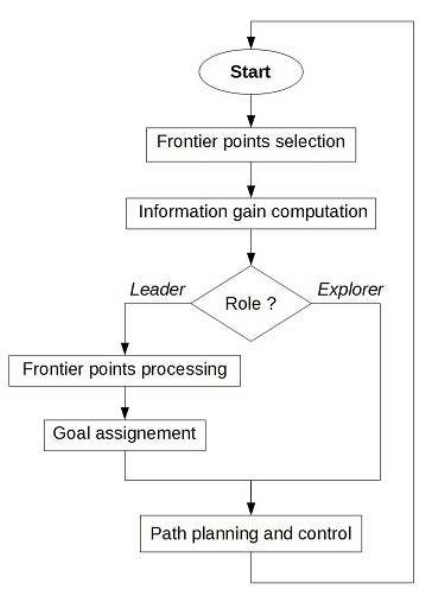
\includegraphics[scale=0.6]{assets/3_1.png}
    \caption{Đề xuất đường ống quá trình thăm dò.}
    \label{fig:3.1}
\end{figure}
Mỗi UAV chọn các điểm biên giới của bản đồ cục bộ được xây dựng trong bước SLAM.Sau đó, nó tính toán thông tin tương ứng của các điểm này.Nếu vai trò của UAV là một \textit{explorer}, nó sẽ thụ động chờ cho đến khi nhận được hướng dẫn;khác, nếu nó hoạt động như một \textit{leader}, Nó sẽ xử lý các điểm biên giới được thu thập, và sẽ chỉ định một mục tiêu cho mỗi robot trong nhóm.Đưa ra một mục tiêu, UAV sẽ lên kế hoạch cho một đường dẫn cụ thể để đạt được nó.\\\\
Trong các bước này, cấu trúc bản đồ phát triển từ bản đồ lưới 2D dự kiến thu được từ mô-đun bản đồ và bản đồ, thông qua các điểm biên giới trong quá trình lựa chọn biên giới, sau đó các mục tiêu ứng cử viên trong bước xử lý biên giới, đến một tập các mục tiêu được chọn để đạt được.Sự phát triển của cấu trúc bản đồ được minh họa trong hình \ref{fig:3.2}. Thuật toán \ref{alg:3.1} mô tả các bước chính được thực hiện trong quá trình thăm dò.
\begin{algorithm}
    \caption{Chiến lược khám phá để phối hợp đa UAV}
    \label{alg:3.1}
    \begin{algorithm}[1]
        \STATE Từ ô $\mathbf{l}_l \in \mathcal{L}$, Chọn điểm biên giới $\mathbf{f}_{i,j} \in \mathcal{F}$ và tính toán thông tin tương ứng của họ $\mathit{\mathbf{I}}(\mathbf{f}_{i,j})$.
        \STATE Xử lý điểm biên giới. $\mathbf{f}_{i,j}$ để có được mục tiêu ứng cử viên $\mathbf{t}_k \in \mathcal{G}$ (Xem thuật toán \ref{alg:3.2})
        \STATE Chỉ định UAV$_i$ với mục tiêu $k$ (Xem thuật toán \ref{alg:3.2}).
        \STATE Gửi mục tiêu đến các robot tương ứng.
    \end{algorithm}
\end{algorithm}
\begin{figure}[H]
    \centering
    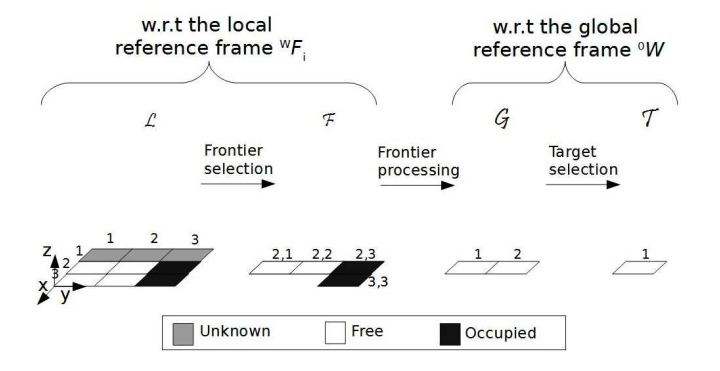
\includegraphics[scale=0.4]{assets/3_2.png}
    \caption{Tiến hóa cấu trúc bản đồ trong quá trình thăm dò: Từ các ô 2D $\mathcal{L}$ đến Ô biên giới 2D. $\mathcal{F}$ để ứng cử viên biên giới / điểm $\mathcal{G}$ (mục tiêu ứng viên) đến 2D ô mục tiêu / điểm $\mathcal{T}$.}
    \label{fig:3.2}
\end{figure}
\subsection{Lựa chọn điểm biên giới}
Quá trình lựa chọn biên giới được sử dụng để định nghĩa biên giới của các vùng bị giới hạn bởi các chướng ngại vật hoặc không gian không xác định (xem hình \ref{fig:3.3}).
\begin{figure}[H]
    \centering
    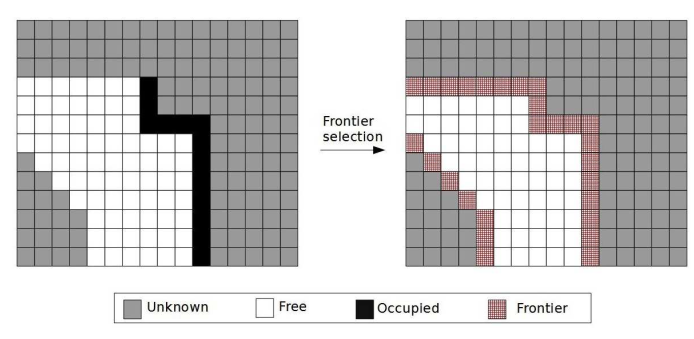
\includegraphics[tỉ lệ=0.4]{assets/3_3.png}
    \caption{Các tế bào biên giới / điểm lựa chọn bản đồ lưới phòng chiếm 2D.}
    \label{fig:3.3}
\end{figure}
Các tế bào biên giới. $\mathbf{f}_{i,j} \in \mathcal{F}$ được chọn từ tập hợp các ô $\mathcal{L}(\mathcal{F}\subset \mathcal{L})$ sao cho họ là:
\begin{itemize}
    \item Miễn phí $\mathbf{l}_f$ và liền kề không rõ.
    \item Dán nhãn là chiếm đóng $\mathbf{l}_o$ . Các ô bị chiếm đóng $\mathbf{l}_o$ được coi là các tế bào biên giới để có thể thực hiện xử lý biên giới trong bước tiếp theo.Chúng không thể được chọn làm mục tiêu và sẽ bị loại bỏ sau.
\end{itemize}
Tại hình \ref{fig:3.2}, Các ô biên giới là: $\mathbf{l}_f(2,1)$,$\mathbf{l}_f(2,2)$ , $\mathbf{l}_f(2,3)$, và $\mathbf{l}_f(3,3)$. Vì vậy, đối với một cụm $\mathcal{C}$ chứa UAV$_i$ , các biên giới là:
\begin{algorimth} \label{eq:3.1}
    \mathcal{F}=\{\mathbf{f}_{i,1}(2,1),\mathbf{f}_{i,2}(2,2),\mathbf{f}_{i,3}(2,3),\mathbf{f}_{i,4}(3,3)\}
\end{algorimth}
\subsection{Thông tin đạt được tính toán}
Trong các phương pháp thăm dò dựa trên biên giới, chỉ có các tế bào liền kề với những tế bào chưa biết có thể được thực hiện dưới dạng các điểm biên giới ứng cử viên và có khả năng sẽ được chọn làm mục tiêu.Qua đó, mức tăng thông tin được liên kết với từng người trong số chúng để ước tính tiện ích tiếp cận từng biên giới.Việc đạt được thông tin tương ứng này có thể được thực hiện trong cách phân cách dirent erent tùy thuộc vào mục đích nhiệm vụ.Tác giả trong \cite{burgard2005coordinated} Đề xuất sử dụng chức năng xác suất để giảm giá trị không đổi được chỉ định có tính đến khoảng cách tương đối với tư thế của UAV.Chiến lược này là chung và không tính đến các ô được cập nhật được cập nhật.Cách tiếp cận được đề xuất trong \cite{heng2015efficient} FF ECTS, để đạt được thông tin, số lượng ô không xác định và không bị chặn trong chế độ xem FrusM của mục tiêu.Phương pháp này phụ thuộc vào ước tính thực tế của thông tin đạt được khi đến thăm tư thế được coi là.Tuy nhiên, nó đòi hỏi nhiều tính toán hơn.\\\\
Trong chiến lược được đề xuất, mức tăng thông tin được phân bổ để nó không xác định lượng các ô không xác định xung quanh mục tiêu (xem hình \ref{fig:3.4}). Nó là một giá trị phi số liệu đếm số lượng các ô được dán nhãn là không xác định l u từ 48 ô xung quanh điểm biên giới.
\begin{figure}[H]
    \centering
    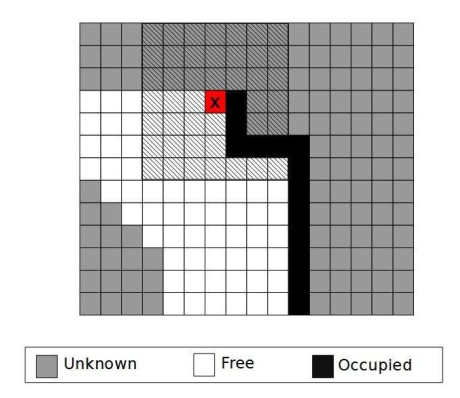
\includegraphics[tỉ lệ=0.4]{assets/3_4.png}
    \caption{Tính toán thông tin đạt được điểm Frontier X (màu đỏ).Các tế bào nở đại diện cho 48 tế bào xung quanh của điểm biên cương \textbf{x}. Sự đạt được thông tin của \textbf{x} là: $\mathbf{I}(x)=25$.}
    \label{fig:3.4}
\end{figure}
\subsection{Xử lý điểm biên giới}
Tất cả các điểm biên giới $\mathbf{f}_{i,j} \in \mathcal{F}$ của UAV$_i$ Trong cụm $\mathcal{C}$ với $i \in [1..n_c]$, được thu thập. Điểm trong $\mathcal{F}$ sau đó được xử lý bằng thuật toán \ref{alg:3.2} để có được các điểm biên giới ứng cử viên được coi là mục tiêu ứng cử viên $\mathbf{t}_k \in \mathcal{G}$ với $k \in [1..n_g]$ (Xem hình \ref{fig:3.2})
\begin{algorimth}[H]
\caption{Thuật toán xử lý biên giới.}
\label{alg:3.2}
\hspace*{\algorithmicindent} \textbf{Input:} Điểm biên giới $\mathbf{f}_{i,j} \in \mathcal{F}$ của UAV$_i$ với $i \in [1..n_c]$. \\
\hspace*{\algorithmicindent} \textbf{Output:} Candidate targets $\mathcal{G}$
\begin{algorithmic}[1]
    \STATE $p_u=\cup_{i=1}^{n_c}\mathbf{f}_{i,j}$.
    \STATE $p_i=\cap_{i=1}^{n_c}\mathbf{f}_{i,j}$.
    \STATE $\mathcal{G}=p_u\setminus p_i$.
    \STATE Xóa các điểm biên giới chướng ngại vật $\mathbf{f}_{i,j}(x,y)=\mathbf{l}_o(x,y)$ from $\mathcal{G}$.
    \RETURN $\mathcal{G}$.
\end{algorithmic}
\end{algorithm}
Hình \ref{fig:3.5} Hiển thị một ví dụ về xử lý biên giới với hai bản đồ của UAV để có được các mục tiêu ứng cử viên.Các điểm biên giới của chướng ngại vật $\mathbf{f}_{i,j}(x,y)=\mathbf{l}_o(x,y)$ – Được dán nhãn là chiếm đóng - chỉ được giữ để tính toán giao điểm của các điểm biên cương.Chỉ các ô Frontier miễn phí $\mathbf{l}_f$ có thể được coi là mục tiêu ứng cử viên.\\\\
Khi sử dụng điểm biên giới cục bộ thay vì bản đồ cục bộ, quy trình biên giới thay thế quy trình khớp bản đồ trong đó mục tiêu là để xóa các khu vực chồng chéo.Do đó, trong bước xử lý biên giới, các điểm biên giới thuộc các khu vực chồng chéo bị xóa.Do đó, sử dụng điểm biên giới cho phép tiết kiệm bộ nhớ quan trọng.Để tính các điểm biên giới thuộc về các khu vực chồng chéo (các bước 1, 2 và 3 trong thuật toán \ref{alg:3.2}), Chúng tôi đề xuất hai cách tiếp cận với các hình dạng lồi và các giả định hình dạng lõm.
\subsubsection{Cách tiếp cận đầu tiên: Bản đồ hình convex}
Trong cách tiếp cận này, các hình dạng bản đồ được coi là convex, đơn giản hóa tính toán giao nhau trong thuật toán \ref{alg:3.3}. Hình \ref{fig:3.6} Hiển thị hai ví dụ về việc áp dụng thuật toán xử lý biên giới trong khi giả sử các hình lồi với hai và ba bản đồ của UAV.\\\\
Thuật toán này tương đối dễ dàng để áp dụng, nhưng kết quả cho thấy rằng nó không hoạt động tốt.Giả định lồi dẫn đến một số điểm biên giới chồng chéo sai.Do đó, một số khu vực chưa biết sẽ không được truy cập vì các điểm tương ứng của chúng được gỡ bỏ và do đó, sẽ không được chỉ định là mục tiêu.
\subsubsection{Cách tiếp cận thứ hai: Bản đồ hình dạng lõm}
Trong cách tiếp cận thứ hai, chúng tôi đưa ra giả định về các hình dạng lõm cho bản đồ của UAV để tính toán giao điểm của chúng trong thuật toán \ref{alg:3.4}. Hình \ref{fig:3.7} Hiển thị hai ví dụ về việc áp dụng thuật toán xử lý biên giới trong khi giả sử các hình lồi với hai và ba bản đồ của UAV.
\begin{figure}[H]
    \centering
    \begin{subfigure}[H]{0.6\linewidth}
        \centering
        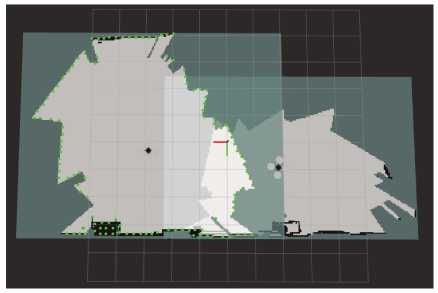
\includegraphics[width=\linewidth]{assets/3_5_a.png}
        \caption{{Frontiers $\mathbf{f}_{1,j}$ of UAV$_1$}}
        \label{fig:3.5a}
    \end{subfigure}
    \begin{subfigure}[H]{0.6\linewidth}
        \centering
        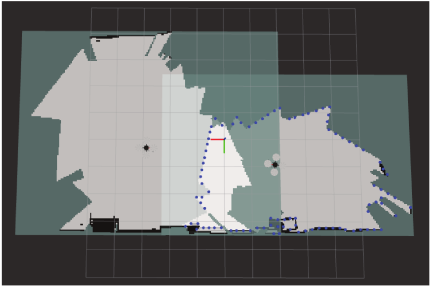
\includegraphics[width=\linewidth]{assets/3_5_b.png}
        \caption{{Frontiers $\mathbf{f}_{2,j}$ of UAV$_2$}}
        \label{fig:3.5b}
    \end{subfigure}
    \begin{subfigure}[H]{0.6\linewidth}
        \centering
        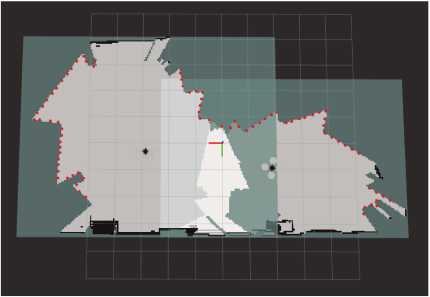
\includegraphics[width=\linewidth]{assets/3_5_c.png}
        \caption{{Candidate targets $\mathcal{G}$}}
        \label{fig:3.5c}
    \end{subfigure}
    \caption{Ví dụ xử lý điểm biên giới: (a) và (b) đại diện cho các điểm biên giới của UAV$_1$ và UAV$_2$, tương ứng. (c) đại diện cho các mục tiêu ứng cử viên.Quá trình này bao gồm loại bỏ các điểm biên giới thuộc về các khu vực chồng chéo, và những điểm nằm liền kề với các chướng ngại vật.}
    \label{fig:3.5}
\end{figure}
\begin{algorithm}[H]
    \caption{Thuật toán tính toán giao nhau với giả định hình dạng lồi.}
    \label{alg:3.3}
    \hspace*{\algorithmicindent} \textbf{Input:} $Vect1, Vect2$ \\
    \hspace*{\algorithmicindent} \textbf{Output:} $Vect\_Final$
    \begin{algorithmic}[1]
        \FOR {$i \in Vect1$}
        \STATE $inf = 0, sup = 0$
        \FOR{ $j \in Vect2$}
        \IF {$Vect1(i).x < Vect2(i).x$}
        \STATE $inf++$;
        \ELSE
        \STATE $sup++$;
        \ENDIF
        \ENDFOR
        \IF {$inf>0$ and $sup>0$}
        \STATE $Vect\_inter.push\_back(Vect1(i))$
        \ENDIF
        \ENDFOR
        \FOR{$i \in Vect\_inter$}
        \STATE $inf=0,sup=0$;
        \FOR{$j \in Vect2$}
        \IF {$|Vect\_inter(i).x-Vect2(i).x| <0.5$}
        \STATE $inf++$;
        \ELSE
        \STATE $sup++$;
        \ENDIF
        \ENDFOR
        \IF {$inf>0$ and $sup>0$}
        \STATE $Vect\_Final.push\_back(Vect\_inter(i))$
        \ENDIF
        \ENDFOR
    \end{algorithmic}
\end{algorithm}
\begin{figure}[H]
    \centering
    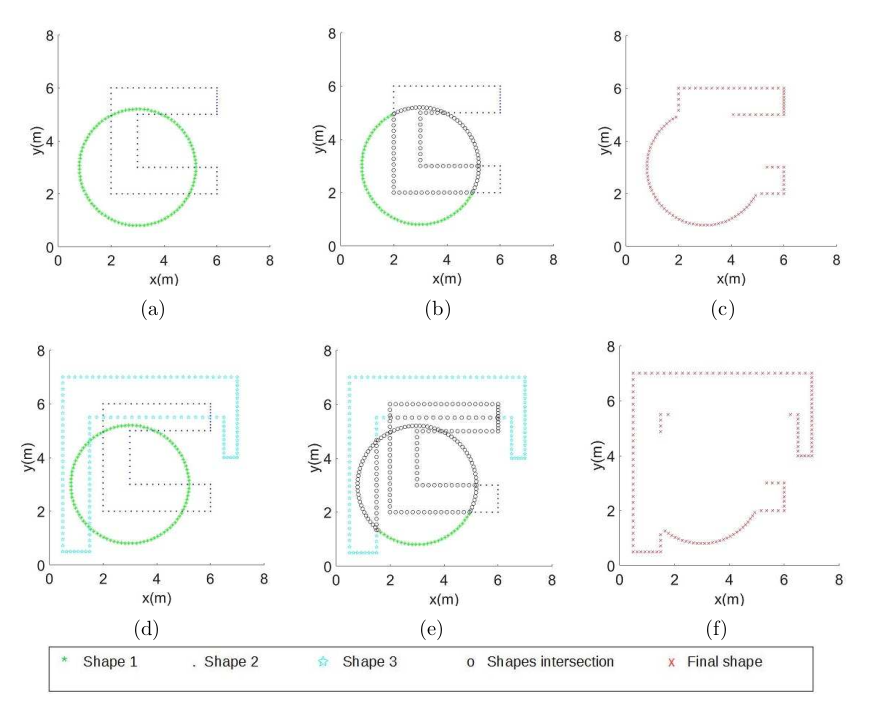
\includegraphics[scale=0.4]{assets/3_6.png}
    \caption{Điểm biên giới xử lý Wile giả định hai hình dạng bản đồ lồi trong dòng đầu tiên và ba trong dòng thứ hai.(a) và (d) biểu thị hai và ba hình dạng bản đồ lồi, tương ứng;(b) và (e) đại diện cho các điểm biên cương theo chồng chéo (giao lộ);và (c) và (f) đại diện cho các điểm biên giới thu được sau khi xử lý (hình dạng nal).}
    \label{fig:3.6}
\end{figure}
\begin{algorithm}[H]
    \caption{Thuật toán tính toán giao nhau với giả định hình dạng lồi.}
    \label{alg:3.4}
    \hspace*{\algorithmicindent} \textbf{Input:} $Vect1, Vect2$ \\
    \hspace*{\algorithmicindent} \textbf{Output:} $Vect\_Final$
    \begin{algorithmic}[1]
        \FOR {$i \in Vect1$}
        \STATE $inf = 0, sup = 0$
        \FOR{ $j \in Vect2$}
        \IF {$Vect1(i).x < Vect2(i).x -0.5$}
        \STATE $inf++$;
        \ELSIF {$Vect1(i).x>Vect2(i).x+0.5$}
        \STATE $sup++$;
        \ELSE
        \STATE $eq++$;
        \ENDIF
        \ENDFOR
        \IF {$inf>0$ and $sup>0$ or $eq>0$}
        \STATE $Vect\_inter.push\_back(Vect1(i))$
        \ENDIF
        \ENDFOR
        \FOR{$i \in Vect\_inter$}
        \STATE $inf=0,sup=0, eq=0$;
        \FOR{$j \in Vect2$}
        \IF {$|Vect\_inter(i).y-Vect2(i).y| <0.5$}
        \IF {$Vect\_inter(i).x<Vect2(i).x-0.5$}
        \STATE $inf++$;
        \ELSIF {$Vect1(i).x>Vect2(i).x+0.5$}
        \STATE $sup++$;
        \ELSE
        \STATE $eq++$;
        \ENDIF
        \ENDIF
        \ENDFOR
        \IF {($inf>0$ and $sup>0$) or $eq>0$}
        \STATE $Vect\_Final.push\_back(Vect\_inter(i))$
        \ENDIF
        \ENDFOR
    \end{algorithmic}
\end{algorithm}
\begin{figure}[H]
    \centering
    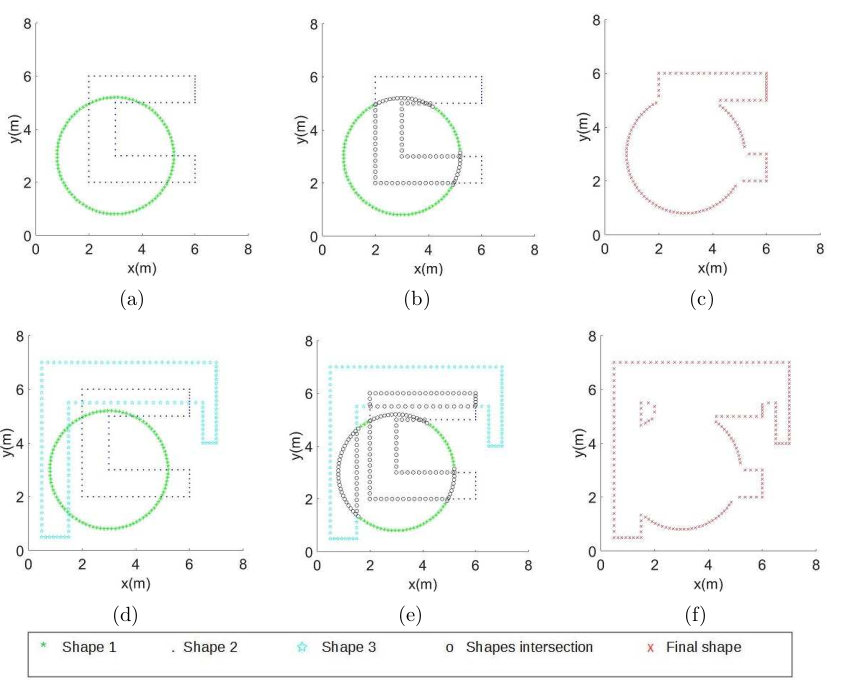
\includegraphics[scale=0.4]{assets/3_7.png}
    \caption{Điểm biên giới xử lý Wile giả định hai hình dạng bản đồ lõm trong dòng đầu tiên và ba trong dòng thứ hai.(a) và (d) biểu thị hai và ba hình dạng bản đồ lồi, tương ứng;(b) và (e) đại diện cho các điểm biên cương theo chồng chéo (giao lộ);và (c) và (f) đại diện cho các điểm biên giới thu được sau khi xử lý (hình dạng nal).}
    \label{fig:3.7}
\end{figure}
Kết quả cho thấy chỉ các điểm biên giới trong các khu vực chồng chéo được loại bỏ.Ngay cả khi một số điểm biên giới mơ hồ được đặt trong / bên trong hình dạng toàn cầu - có thể gây nhầm lẫn -, chúng không bị xóa.Thuật toán này, giả sử các hình dạng lõm, thực hiện tốt hơn so với trước đó giả định hình dạng lồi.Do đó, đối với chế biến biên giới, hình dạng của bản đồ địa phương được giả định lõm.
\subsubsection{Chức năng tiện ích}
Chức năng tiện ích được đề xuất trong EQ. \ref{eq:3.2} Nhằm mục đích tăng đồng thời tỷ lệ khu vực được khám phá và để giảm khoảng cách của từng UAV đến mục tiêu tương ứng.Chức năng này cũng xem xét trung bình khoảng cách giữa mỗi robot trong nhóm và mục tiêu này để tối đa hóa khoảng cách giữa các robot.
\begin{equation}
    \mathbf{U}(UAV_i,t_j)=\mathbf{I}(t_j)exp(-\lambda.(dmin(\mathbf{P}_i,\mathbf{t}_j)+\frac{n_c-1}{d_{tot}})),
\end{equation}
Nơi UAV tôi là robot được coi là, $\mathbf{t}_j \in \mathcal{G}$ và $\mathbf{I}(\mathbf{t}_j)$ tương ứng là mục tiêu ứng viên và mức tăng thông tin tương ứng của nó, $\lambda \in [0,1]$ là một tham số Trade-o ff, $n_c$ là số lượng UAV trong cụm $\mathcal{C}$, and $d_{tot} = \sum_{k=1, k\neq i}^{n_c}(dmin(\mathbf{P}_k),\mathbf{t}_j) $ là tổng của khoảng cách tối thiểu từ UAV$_k$'s tư thế $\mathbf{P}_k$ đến mục tiêu ứng viên $j$. Chức năng tiện ích được đề xuất được truyền cảm hứng từ \cite{heng2015efficient} và nó đã được trình bày trong các tác phẩm của chúng tôi \cite{mahdoui2017cooperative},\cite{mahdoui2018cooperative}. Hàm này thực hiện giao dịch giữa OF FF giữa khám phá nhanh chóng và một bản đồ chính xác bằng cách sử dụng tham số điều chỉnh $\lambda$. Từ hình \ref{fig:3.8}, Chúng ta có thể nhận thấy rằng lớn hơn $\lambda$, Khoảng cách ít quan trọng hơn $d_{tot}$. Do đó, một cách chính xác được ưa chuộng về việc thăm dò nhanh chóng và ngược lại.\\\\
Về trường hợp đa UAV, chức năng tiện ích dựa trên trung bình khoảng cách hàng xóm.Như thể hiện trong hình \ref{fig:3.8}, với một thông tin đạt được $\mathbf{I}(\mathbf{t}_j)=25$ và ba UAV trong cụm $(n_c=3)$; Một khoảng cách ngày càng tăng của UAV đến mục tiêu sẽ làm giảm chức năng tiện ích.Trong khi đó, khoảng cách trung bình lớn hơn so với các UAV khác w.r.t.đến mục tiêu, tiện ích càng nhiều.Vì vậy, chức năng có xu hướng chọn mục tiêu gần nhất với UAV được coi là;Nhưng đồng thời, xa nhất từ những người khác.\\\\
Trong trường hợp một UAV duy nhất, chức năng tiện ích (xem EQ. \ref{fig:3.3}) Có xu hướng chọn mục tiêu gần nhất với mức tăng tối đa thông tin:
\begin{equation}
    \mathbf{U}(UAV_i,\mathbf{t}_j)=\mathbf{I}(\mathbf{t}_j)exp(-\lambda.(dmin(\mathbf{P}_j,\mathbf{t}_j))),
\end{equation}
Thông số $d_{tot} = \sum_{k=1, k\neq i}^{n_c}(dmin(\mathbf{P}_k,\mathbf{t}_j)) $ đại diện cho tổng khoảng cách tối thiểu giữa mục tiêu $\mathbf{t}_j$ và các vị trí của hàng xóm $\mathbf{P}_k$ với $k \in [1..n_c]\setminus i$. Vì thế nếu $\mathbf{t}_j$ Có các UAV lân cận quá xa, chức năng tiện ích sẽ tăng lên, vì vậy T J có nhiều khả năng được chọn.\\\\
Mục tiêu trong chức năng tiện ích là tối đa hóa $d_{tot}$ . Chúng tôi phân biệt hai trường hợp $d_{tot}$ có thể quá gần bằng 0 hoặc bằng nó:
\begin{figure}[H]
    \centering
    \begin{subfigure}[H]{0.4\linewidth}
        \centering
        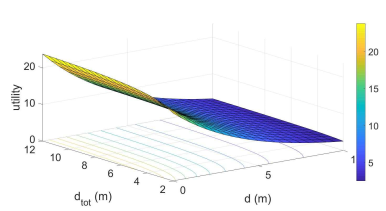
\includegraphics[width=\linewidth]{assets/3_8_a.png}
        \caption{{$\lambda=0.2$}}
        \label{fig:3.8a}
    \end{subfigure}
    \begin{subfigure}[H]{0.4\linewidth}
        \centering
        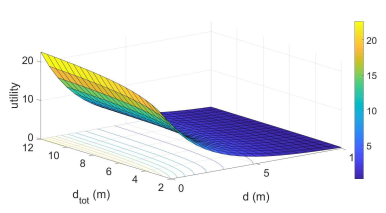
\includegraphics[width=\linewidth]{assets/3_8_b.png}
        \caption{{$\lambda=0.4$}}
        \label{fig:3.8b}
    \end{subfigure}
    \begin{subfigure}[H]{0.4\linewidth}
        \centering
        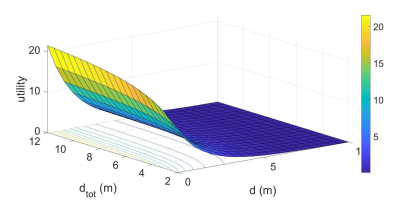
\includegraphics[width=\linewidth]{assets/3_8_c.png}
        \caption{{$\lambda=0.6$}}
        \label{fig:3.8c}
    \end{subfigure}
    \begin{subfigure}[H]{0.4\linewidth}
        \centering
        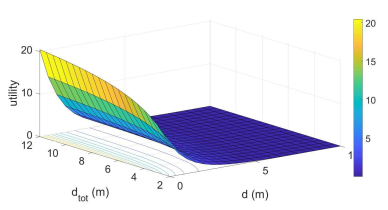
\includegraphics[width=\linewidth]{assets/3_8_d.png}
        \caption{{$\lambda=0.8$}}
        \label{fig:3.8d}
    \end{subfigure}
    \caption{{Hành vi chức năng tiện ích: $\mathbf{I}(t_j)=25, n_c=3, d_{tot} = \sum_{k=1, k\neq i}^{n_c}(dmin(\mathbf{P}_k,\mathbf{t}_j))$. Khoảng cách trung bình của khác UAVs $d_{tot}$ có giá trị tối thiểu khác với số 0 kể từ khi $n_c$ khác với 0 quá.}}
    \label{fig:3.8}
\end{figure}
\begin{itemize}
    \item Không có hàng xóm.Trong trường hợp này, có một UAV trong FL EET: $n_c=1$. Chức năng tiện ích trong EQ. \ref{eq:3.3} được sử dụng.
    \item Mục tiêu ứng cử viên $\mathbf{t}_j$ và các vị trí của hàng xóm $\mathbf{P}_k$ với $k \in [1..n_c]\setminus i$ gần như bối rối (quá gần nhau).Trong trường hợp này $\mathbf{t}_j$ ít có khả năng được chọn.
\end{itemize}
Tuy nhiên, tham số này $d_{tot}$ có thể có giá trị cao khi:
\begin{itemize}
    \item Có một UAV quá xa $\mathbf{t}_j$.
    \item Có một số UAV với khoảng cách tương đối ngắn từ $\mathbf{t}_j$.
\end{itemize}
Vì vậy, để tránh những tình huống mơ hồ này, trung bình của $d_{tot}$ được xem xét bằng cách sử dụng $\frac{n_c}{d_{tot}}$.
\subsection{Quy trình phân công mục tiêu}
Để thực hiện phân công UAV-to-nhắm mục tiêu thích hợp, tiện ích tiếp cận từng biên giới ứng cử viên được xem xét.Quá trình phân công mục tiêu được mô tả trong Algo. \ref{alg:3.5}.\\\\
Cho mỗi UAV$_i$ , Các tiện ích để đạt được tất cả các mục tiêu ứng cử viên được tính toán.Mục tiêu $\mathbf{t}_g$ tối đa hóa tiện ích được tính toán và, bài tập $\theta(UAV_i,\mathbf{t}_g)$ được thực hiện.Sau đó, các mục tiêu ứng cử viên còn lại $\mathcal{G}\setminus \mathcal{T}$ được lên kế hoạch để tránh để chọn một mục tiêu quá gần $\mathbf{t}_g$ , trong lần lặp tiếp theo.Cũng thế, $\mathbf{t}_g$ được gỡ bỏ khỏi $\mathcal{G}$ để ngăn chặn việc chỉ định cùng một mục tiêu cho di ff robot erent erent.Quá trình chuyển nhượng này được thực hiện cho các UAV có sẵn trong $\mathcal{C}$ theo cách tuần tự cho đến khi nhận được tất cả các mục tiêu được chỉ định $\mathbf{t}_g \in \mathcal{T}$ với $g \in [1..n_t]$ (Xem hình \ref{fig:3.2})
\begin{algorithm}[H]
    \caption{Thuật toán gán mục tiêu.}
    \label{alg:3.5}
    \hspace*{\algorithmicindent} \textbf{Input:} {Mục tiêu ứng viên $\mathbf{t}_k \in \mathcal{G}, k \in [1..n_g]$ và thông tin tương ứng của họ đạt được $\mathbf{U}(\mathbf{t}_k)$, poses $\mathbf{P}_i$ của tất cả các robot trong cụm được coi là $\mathcal{C}$.}\\
    \hspace*{\algorithmicindent} \textbf{Output:} {$\theta(UAV_i,\mathbf{t}_g)$ phân công UAV$_i$ với mục tiêu $g$.}
    \begin{algorithmic}[1]
        \STATE $\mathcal{T}=\theta$
        \WHILE{Không có mục tiêu cho UAV$_i$}
        \STATE Tính toán tiện ích tương ứng của nó để đạt được mỗi mục tiêu ứng cử viên còn lại $\mathbf{U}(UAV_i,\mathbf{t}_k)$ với $\mathbf{t}_k \in \mathcal{G}\setminus \mathcal{T}$.
        \STATE $t_g=argmax_{t_k \in \mathcal{G}\setminus \mathcal{T}}(\mathbf{U}(UAV_i,\mathbf{t}_k))$.
        \STATE Lên lịch để đạt được thông tin của các ứng cử viên còn lại $\mathbf{t}_k \in \mathcal{G} \setminus \mathcal{T}$.
        \STATE $\mathcal{T}=\mathcal{T}\cup t_g$.
        \ENDWHILE
        \RETURN $\theta(UAV_i, \mathbf{t}_g)$ assignment.
    \end{algorithmic}
\end{algorithm}
\subsubsection{Stop condition}
Quá trình lựa chọn mục tiêu được thực hiện bởi mỗi cluster/group-\textit{leader} (if $n>n-c$ ) hoặc đội tàu- \textit{leader} (if $n=n_c$). Nhiệm vụ này nhằm mục đích, hợp tác, phân phối robot trong môi trường để khám phá đồng thời di ff erent khu vực không xác định.Miễn là các điểm biên giới ứng cử viên vẫn có sẵn, \textit{leader} tiếp tục gán mục tiêu cho \textit{explorers} và họ cố gắng đạt được mục tiêu được giao.Khi mà \textit{leader} Thông báo rằng không có mục tiêu ứng cử viên nào còn lại, điều đó có nghĩa là tất cả các môi trường đã được khám phá thành công và nhiệm vụ được thực hiện.Vì vậy, nó phải gửi lại cho \textit{explorers} một sự thừa nhận để ngăn chặn họ giả định mất giao thông.
\subsubsection{Loop rate}
Quá trình phân công mục tiêu được thực hiện tại mỗi vòng lặp.Tần suất gán các mục tiêu ảnh hưởng đến thời gian và sự nghiêm trọng của FFI của nhiệm vụ.Trong một cách tiếp cận phân tán, ngay khi UAV đạt được mục tiêu hiện tại, nó sẽ chọn một mục tiêu mới mà không cần tham khảo ý kiến người khác.Trong một cách tiếp cận tập trung, UAV đầu tiên để đạt được mục tiêu hiện tại phải đợi cho đến khi những người khác đạt được mục tiêu tương ứng.Đây có thể là một vấn đề ngay khi một trong số họ thất bại hoặc rời khỏi nhiệm vụ.Một khả năng khác là bắt đầu gán các mục tiêu sau khi UAV đạt được mục tiêu.Nhưng điều này có thể tạo ra các nhiệm vụ không đầy đủ.Trong chiến lược đề xuất, tần suất phân công hoặc tỷ lệ vòng lặp $r$ là fi ned tùy thuộc vào trung bình thời gian để đạt được một mục tiêu (Xem Eq. \ref{eq:3.4}).
\begin{equation} \label{eq:3.4}
    r \in [\frac{s}{v_{i,max}},\frac{s}{v_{i,min}}]
\end{equation}
Ở $s$ là phạm vi cảm biến tối đa và $v_i$ là vận tốc của UAV.
\subsubsection{Lên lịch để đạt vớiược thông tin}
Tăng thông tin của từng mục tiêu ứng cử viên còn lại $\mathbf{I}(\mathbf{t}_k)_{t-1}$ tại thời điểm $t-1$ với $\mathbf{t}_k \in \mathcal{G} \setminus \{t_g\}$, thuộc về phạm vi ngưỡng $[r_{min} , r_{max} ]$, được lên kế hoạch tại thời điểm $ t $ tùy theo khoảng cách của nó w.r.t.mục tiêu $t_g$ , sử dụng Eq. \ref{eq:3.5}. Hình \ref{fig:3.9} đại diện cho một ví dụ về hình dạng chức năng được sử dụng để lên lịch để đạt được thông tin.Ví dụ cho thấy một hàm Gaussian với biên độ tương ứng với giá trị tối đa thông tin;một trung tâm tương ứng với vị trí mục tiêu $(\mathbf{t}_g(x), \mathbf{t}_g(y))$; và $\sigma_x$ và $\sigma_y$ nó lan rộng blob trong $x$ và $y$ trục, tương ứng.
\begin{figure}[H]
    \centering
    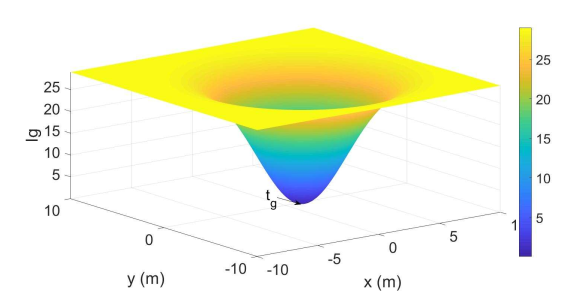
\includegraphics[scale=0.6]{assets/3_9.png}
    \caption{Ví dụ về chức năng hình dạng để lên lịch để đạt được thông tin($\mathbf{I}(\mathbf{t}_k)_{t-1}=29,(\mathbf{t}_g(x),\mathbf{t}_g(y))=(1.25,-0.275), \sigma_x=\sigma_y=3$).}
    \label{fig:3.9}
\end{figure}
\begin{equation}\label{eq:3.5}
    \mathbf{I}(\mathbf{t}_k)_t=\mathbf{I}(\mathbf{t}_k)_{t-1}(1-exp(-(\frac{(\mathbf{t}_k(x)-\mathbf{t}_g(x))^2}{2.\sigma_x^2}+\frac{(\mathbf{t}_k(y)-\mathbf{t}_g(y))^2}{2.\sigma_y^2}))),
\end{equation}
Ở $\mathbf{t}_k(x)$ and $\mathbf{t}_k(y)$ là tọa độ mục tiêu ứng cử viên còn lại; $\mathbf{t}_g(x)$ và $\mathbf{t}_g(y)$ là tọa độ mục tiêu;và $\sigma_x$ và $\sigma_y$ là những lây lan của blob.Khoảng cách của điểm biên giới nhỏ hơn $\mathbf{t}_k$ w.r.t.mục tiêu $\mathbf{t}_g$, sự tăng thông tin càng nhỏ.Khi giảm mức tăng thông tin, các mục tiêu ứng cử viên ít có khả năng được chọn và do đó, robot đảm bảo một khoảng cách nhất định trong số các mục tiêu trong tương lai của họ.
\subsection{Lập kế hoạch và kiểm soát đường dẫn}
AS được giải thích trong Phần 5.2 của Chương 1, UAV được giả định là điều hướng trong môi trường 2D đơn giản với A FI XED $z$ giá trị. Khối \textbf{6} Trong Hình 1.6 chịu trách nhiệm lên kế hoạch đường dẫn đến mục tiêu đã chọn và cố gắng tiếp cận nó.Những nhiệm vụ này được đảm bảo bởi \textit{move} căn cứ\footnote{Nguồn: \url{http://wiki.ros.org/move_base}} gói.\\\\
Đối với nhiệm vụ điều hướng, mỗi UAV duy trì một công cụ lập kế hoạch địa phương và toàn cầu cùng với một costmap địa phương và toàn cầu.COSTMAP là một lưới ô 2D $\mathcal{L}$ Với bổ sung trong fl ation bao gồm việc truyền các giá trị chi phí từ các tế bào bị chiếm đóng và giảm chúng bằng khoảng cách.CostMap toàn cầu có kích thước của bản đồ của UAV trong khi đó, costmap địa phương có một cửa sổ di chuyển kích thước fi xed.Đưa ra một điểm khởi đầu - tư thế hiện tại - và điểm cuối - Mục tiêu được chỉ định - trong Costmap toàn cầu, công cụ lập kế hoạch toàn cầu tạo ra một kế hoạch sử dụng chức năng điều hướng được tính bằng thuật toán Dijkstra \cite{dijkstra1959note}. Nó bao gồm sau các tế bào miễn phí liền kề cho đến khi đạt được mục tiêu.Sau đó tính đến chi phí địa phương, công cụ lập kế hoạch cục bộ tạo ra các lệnh vận tốc cho căn cứ di động của UAV.Một hành vi quay trở lại cũng được thực hiện khi cần thiết để xóa chế độ xem của robot.\\\\
Mục tiêu được chỉ định bởi \textit{leader} được đảm bảo là thuộc về một khu vực không xác định bằng cách sử dụng chiến lược thăm dò.Quá trình lập kế hoạch quỹ đạo được thực hiện tại địa phương trên mỗi robot.Và vì UAV không trao đổi bản đồ địa phương của họ cũng như hợp nhất chúng, họ có khả năng xem lại các khu vực đã khám phá trong khi theo đường dẫn theo kế hoạch.Để giảm thiểu các vùng chồng chéo này trong quá trình điều hướng, ưu tiên được đưa ra cho các điểm biên giới $\mathbf{f}_{i,j}$ là một mục tiêu cho UAV$_i$ ngoài UAV$_k$ với $k \neq i$. Điều này giúp UAV duy trì cùng một hướng trong quá trình thăm dò.Các \textit{move} Gói cơ sở là một ngăn xếp điều hướng 2D.Tuy nhiên, để tránh trôi dạt trên $z$ Trục, một lệnh điều khiển được thêm vào để giữ tĩnh $z$ độ cao (Xem hình \ref{fig:3.10}).
\begin{figure}[H]
    \centering
    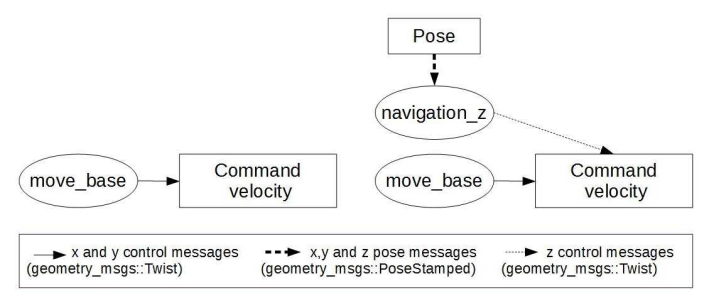
\includegraphics[scale=0.4]{assets/3_10.png}
    \caption{Từ ngăn xếp điều hướng 2D (trái) sang 3D (phải).Các \textit{navigation} z là một quá trình ROS được phát triển để cung cấp một lệnh điều khiển trên trục Z.}
    \label{fig:3.10}
\end{figure}
\section{Kết quả và thảo luận}
Mô phỏng đã được thực hiện để đánh giá chiến lược thăm dò được đề xuất.Các thử nghiệm bổ sung trong khi sử dụng bản địa hóa tương đối đã được thực hiện để đo lường hiệu suất hệ thống.Các mô phỏng được thực hiện bằng Hệ điều hành Robot (ROS) chạy trên máy I7 Linux 2.60GHz.Đối với mô phỏng bốn cánh quạt, mô hình ar-drone\footnote{Nguồn: \url{http://wiki.ros.org/ardrone_autonomy}} Được trang bị máy ảnh RGB-D theo điều kiện tìm kiếm phía trước, được sử dụng.Một môi trường không xác định được tạo ra bằng cách sử dụng \textit{Gazebo} giả lập.Số lượng robot được sử dụng để đánh giá được giới hạn trong ba, tuy nhiên, kiến trúc hệ thống được đề xuất không bị hạn chế với số robot xed.
\subsection{Điều chỉnh thông số}
Đối với một đánh giá EF FF của Chiến lược thăm dò, chúng tôi sẽ chạy một số thử nghiệm để đặt các thông số đầy đủ nhất có liên quan.
\subsubsection{Tham số đánh đổi $\lambda$}
Chức năng tiện ích (xem Eq. \ref{eq:3.2}) được sử dụng trong chiến lược thăm dò có thể được điều chỉnh, sử dụng một tham số thương mại o ff $\lambda$, giữa thăm dò nhanh và tìm kiếm chi tiết về bản đồ.\\\\
Hình \ref{fig:3.11} Hiển thị di ff erent chạy trong khi thay đổi tham số này.Bằng cách tăng lên $\lambda$, Thông tin thu được khi đạt được mục tiêu được ưa chuộng về khoảng cách và do đó, chi phí cho nó và ngược lại.Vì vậy, khi nào $\lambda$ là nhỏ, khoảng cách di chuyển là nhỏ và vì vậy thời gian thăm dò.Mặc dù, một số lần trong nhiệm vụ, giá trị cao của $\lambda$ được nhận thấy để đạt được tỷ lệ thăm dò cao hơn so với những người nhỏ hơn.
\begin{figure}[H]
    \centering
    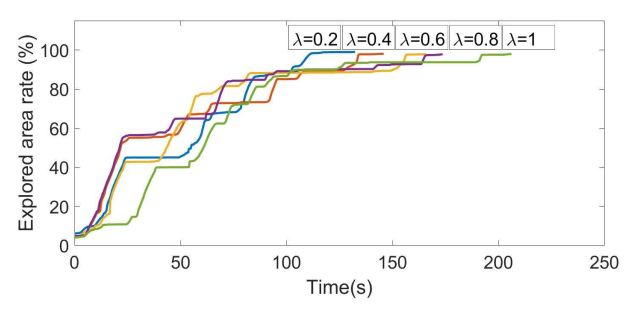
\includegraphics[scale=0.5]{assets/3_11.png}
    \caption{Tác động của việc thay đổi tham số thương mại $\lambda$ qua thời gian thăm dò.}
    \label{fig:3.11}
\end{figure}
\subsubsection{Tỷ lệ vòng lặp $r$}
Tỷ lệ tần số hoặc vòng lặp $r$ Nhiệm vụ mục tiêu cũng có thể là một hiệu suất thời gian thăm dò của FF.Các giá trị của. $r$ thay đổi để tính đến vận tốc robot $\mathbf{v}_i$ và phạm vi tối đa của cảm biến $s$. Tác động của việc thay đổi tỷ lệ vòng lặp được đánh giá trong hình \ref{fig:3.12}.
\begin{figure}[H]
    \centering
    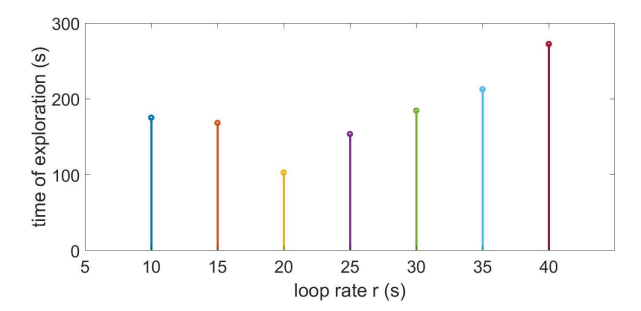
\includegraphics[scale=0.5]{assets/3_12.png}
    \caption{Thời gian khám phá trong khi thay đổi tỷ lệ vòng lặp $r$.}
    \label{fig:3.12}
\end{figure}
Đưa ra một vận tốc robot $\mathbf{v}_i=\{0.1,0.3\}m.s^{-1}$ và một phạm vi cảm biến tối đa $s=4m$, Tốc độ vòng lặp biến dạng trong $r \in [10,40]$. Tham số này không nên quá nhỏ để cho phép robot đạt được mục tiêu;Cũng không quá lớn để ngăn chặn thời gian chờ đợi dài cho nhiệm vụ mục tiêu tiếp theo.
\subsubsection{Thông số chung}
Tùy thuộc vào kết quả trong hình \ref{fig:3.11} và hình. \ref{fig:3.12}, tương ứng, $\lambda$ được đặt thành $0.2$ và $r$ đến $20s$ Để tối đa hóa tỷ lệ khu vực được khám phá trong khi giảm thiểu thời gian nhiệm vụ.Các tham số mô phỏng được tóm tắt trong bảng \ref{tab:3.1}.
\begin{table}[H]
    \centering
    \caption{Thông số chung.}
    \label{tab:3.1}
    \begin{tabular}{|l|l|}\hline
        \makebox[5em]{\textbf{Parameter}}                & \makebox[5em]{\textbf{Value}}
        \\\hline
        RGB-D PROIZONTAL FOV                             & $\pi/ 3$                      \\\hline
        Tham số đánh đổi $\lambda$                       & 0.2                           \\\hline
        Phạm vi tối đa RGB-D $s (m)$                     & 4                             \\\hline
        Khoảng cách tối thiểu giữa các biên giới $d (m)$ & 0.3                           \\\hline
        Độ phân giải lưới chiếm dụng $(m)$               & 0.05                          \\\hline
        Phạm vi để lên lịch $\lg[\sigma_x,\sigma_y] (m)$ & $[3,3]$                       \\\hline
        Tỷ lệ vòng lặp $l (s)$                           & 20                            \\\hline
        Kích thước môi trường $(m^2)$                    & $8 \times 8$                  \\\hline
        Vận tốc tuyến tính. $v_i (m.s^{-1})$             & $[0.1,0.3]$                   \\\hline
        Vận tốc góc cạnh $w_i (rad.s^{-1})$              & $[0.1,0.3]$                   \\\hline
    \end{tabular}
\end{table}
\subsection{Biểu diễn chiến lược khám phá}
Chiến lược thăm dò được đề xuất đã được đánh giá về mặt phân phối robot trong môi trường, tỷ lệ chồng chéo, thời gian thăm dò và toàn bộ khoảng cách di chuyển của mỗi robot.
\subsubsection{Bản đồ tiến hóa trong nhiệm vụ}
Trong khi đạt được mục tiêu được giao nhiệm vụ tương ứng, mỗi robot phụ trách việc tạo bản đồ lưới chi tiết của khu vực đã truy cập để có được bản đồ toàn cầu về môi trường.Hình \ref{fig:3.13} minh họa sự tăng trưởng của bản đồ lưới chiếm dụng 3D được xây dựng lại tại Di Ff Erent Times trong nhiệm vụ.Lưu ý rằng để đạt được $99\%$ của phạm vi bảo hiểm, rất nhiều thời gian được chi tiêu.\\\\
Hình \ref{fig:3.14} Hiển thị sự phát triển của bản đồ lưới địa phương 2D dự kiến tương ứng của hai robot trong một nhiệm vụ thăm dò hợp tác xã.Bản đồ lưới 2D dự kiến toàn cầu cũng được tạo và đại diện để đánh giá (quy trình khớp lưới chiếm dụng được giới thiệu trong thuật toán 2.1 trong Chương 2 được sử dụng).Vị trí ban đầu của robot là $(1,0,0)$ cho UAV$_1$ và $(1,-3,0)$ cho UAV$_2$. Mặc dù có vị trí ban đầu tương đối chặt chẽ, chiến lược được đề xuất e ff ectuly lây lan robot để UAV$_1$ phụ trách bên trái của môi trường và UAV$_2$ của bên phải.
\subsubsection{Frontier điểm tiến hóa trong nhiệm vụ}
Mục tiêu được chọn từ các điểm biên giới ứng cử viên mà các cạnh của một môi trường không được khám phá trước đó.Những ứng cử viên này được chọn từ các điểm biên giới Nal của mỗi UAV trong fl eet (xem hình \ref{fig:3.15}). Trong nhiệm vụ thăm dò, kích thước bản đồ địa phương tăng lên, dẫn đến số lượng điểm biên giới cục bộ ngày càng tăng.Khi bắt đầu thăm dò, số lượng điểm biên giới ứng cử viên tăng lên, nhưng ngay khi thăm dò tiến hóa kịp thời, số lượng của họ giảm.Vào cuối nhiệm vụ, khi tất cả các môi trường được khám phá, không nên để lại điểm biên giới ứng cử viên.
\subsubsection{Quỹ đạo của UAV trong nhiệm vụ}
Hình \ref{fig:3.16} Hiển thị bản đồ được khám phá với các quỹ đạo bằng cách sử dụng một, hai và ba UAV.UAV cố gắng khám phá môi trường đầy đủ trong khi tránh các khu vực đã khám phá.Một cách hợp tác, mỗi UAV phụ trách truy cập một khu vực bằng cách đạt được mục tiêu thuộc về một môi trường không khám phá.Những mục tiêu này được chỉ định bởi \textit{Leader} Ngay cả khi, ngay cả khi các tư thế ban đầu của UAV tương đối gần, E FF vượt qua chúng vào các khu vực chưa biết.Bản đồ toàn cầu bao gồm sự chồng chất của tất cả các bản đồ địa phương của tất cả các UAV.
\begin{figure}[H]
    \centering
    \begin{subfigure}[H]{0.3\linewidth}
        \centering
        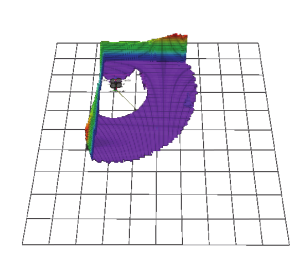
\includegraphics[chiều rộng=\linewidth]{assets/3_13_a.png}
        \caption{{$3\%$ tỉ lệ $(5s).$}}
        \label{fig:3.13a}
    \end{subfigure}
    \begin{subfigure}[H]{0.3\linewidth}
        \centering
        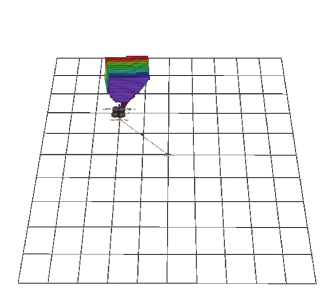
\includegraphics[chiều rộng=\linewidth]{assets/3_13_b.png}
        \caption{{$20\%$ tỉ lệ $(28s).$}}
        \label{fig:3.13b}
    \end{subfigure}
    \begin{subfigure}[H]{0.3\linewidth}
        \centering
        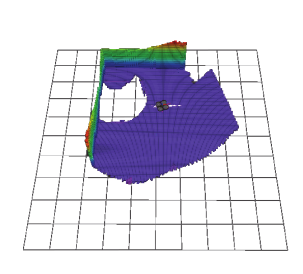
\includegraphics[chiều rộng=\linewidth]{assets/3_13_c.png}
        \caption{{$31\%$ tỉ lệ $(50s).$}}
        \label{fig:3.13c}
    \end{subfigure}
    \begin{subfigure}[H]{0.3\linewidth}
        \centering
        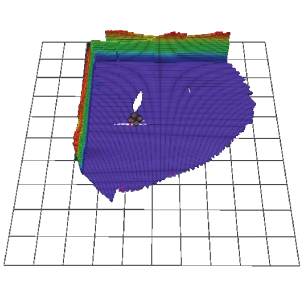
\includegraphics[chiều rộng=\linewidth]{assets/3_13_d.png}
        \caption{{$40\%$ tỉ lệ $(69s).$}}
        \label{fig:3.13d}
    \end{subfigure}
    \begin{subfigure}[H]{0.3\linewidth}
        \centering
        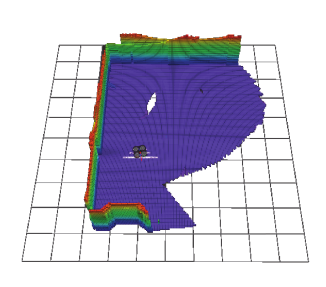
\includegraphics[chiều rộng=\linewidth]{assets/3_13_e.png}
        \caption{{$50\%$ tỉ lệ $(75s).$}}
        \label{fig:3.13e}
    \end{subfigure}
    \begin{subfigure}[H]{0.3\linewidth}
        \centering
        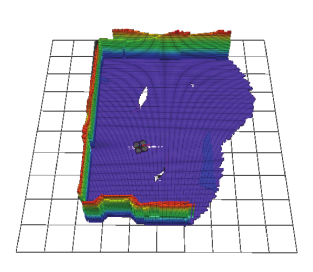
\includegraphics[chiều rộng=\linewidth]{assets/3_13_f.png}
        \caption{{$60\%$ tỉ lệ $(83s).$}}
        \label{fig:3.13f}
    \end{subfigure}
    \begin{subfigure}[H]{0.3\linewidth}
        \centering
        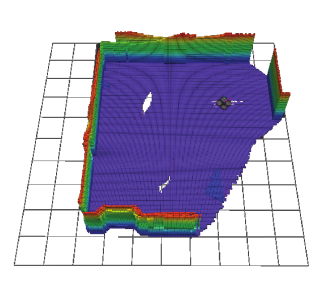
\includegraphics[chiều rộng=\linewidth]{assets/3_13_g.png}
        \caption{{$70\%$ tỉ lệ $(98s).$}}
        \label{fig:3.13g}
    \end{subfigure}
    \begin{subfigure}[H]{0.3\linewidth}
        \centering
        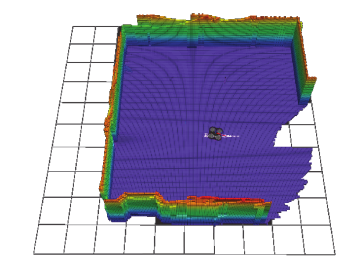
\includegraphics[chiều rộng=\linewidth]{assets/3_13_h.png}
        \caption{{$81\%$ tỉ lệ $(127s).$}}
        \label{fig:3.13h}
    \end{subfigure}
    \begin{subfigure}[H]{0.3\linewidth}
        \centering
        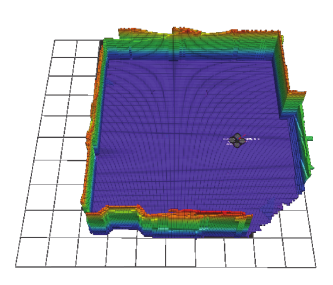
\includegraphics[chiều rộng=\linewidth]{assets/3_13_i.png}
        \caption{{$90\%$ tỉ lệ $(133s).$}}
        \label{fig:3.13i}
    \end{subfigure}
    \begin{subfigure}[H]{0.3\linewidth}
        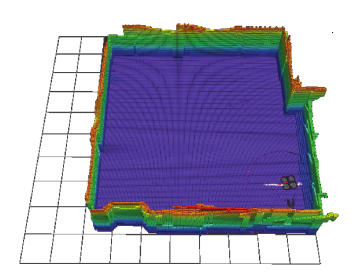
\includegraphics[chiều rộng=\linewidth]{assets/3_13_j.png}
        \caption{{$99\%$ tỉ lệ $(202s).$}}
        \label{fig:3.13j}
    \end{subfigure}
    \caption{Tỷ lệ không gian khám phá trong thời gian cho một UAV.}
    \label{fig:3.13}
\end{figure}
\begin{figure}[H]
    \centering
    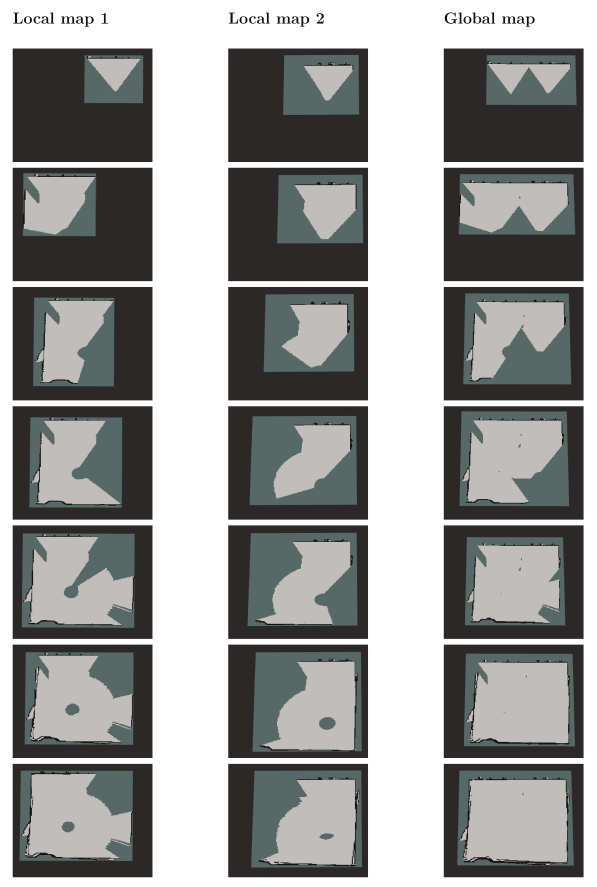
\includegraphics[tỉ lệ=0.5]{assets/3_14.png}
    \caption{Phối hợp thăm dò bằng hai robot.Cột 1, 2 và 3 cho thấy sự phát triển của bản đồ địa phương của UAV$_1$, các UAV$_2$ và bản đồ toàn cầu theo thời gian, tương ứng.}
    \label{fig:3.14}
\end{figure}
\begin{figure}[H]
    \centering
    \begin{subfigure}[H]{0.7\linewidth}
        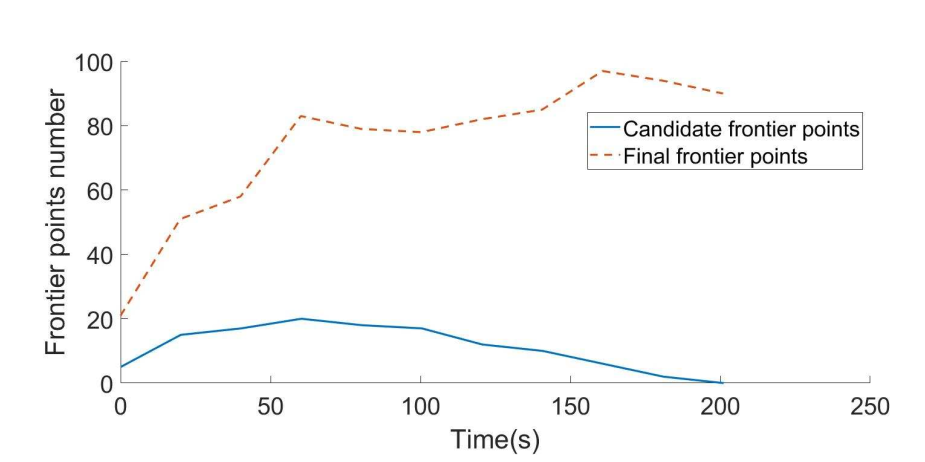
\includegraphics[chiều rộng=\linewidth]{assets/3_15_a.png}
        \caption{{Một UAV.}}
        \label{fig:3.15a}
    \end{subfigure}
    \begin{subfigure}[H]{0.7\linewidth}
        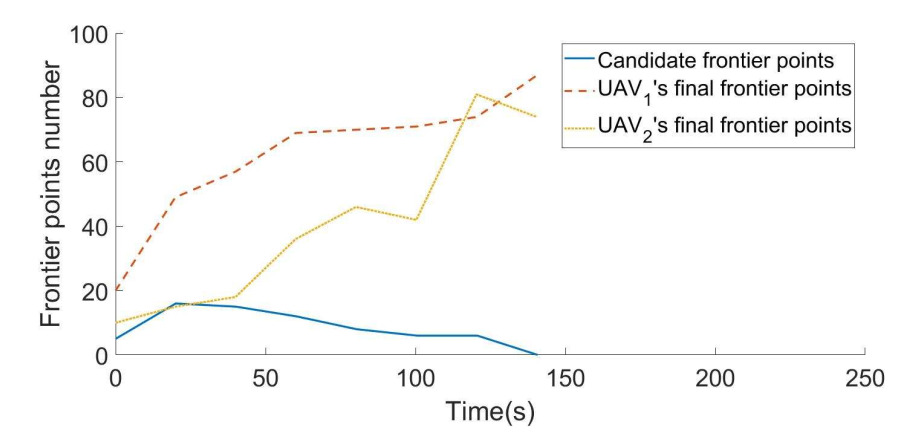
\includegraphics[chiều rộng=\linewidth]{assets/3_15_b.png}
        \caption{{Hai UAV kết hợp.}}
        \label{fig:3.15b}
    \end{subfigure}
    \begin{subfigure}[H]{0.7\linewidth}
        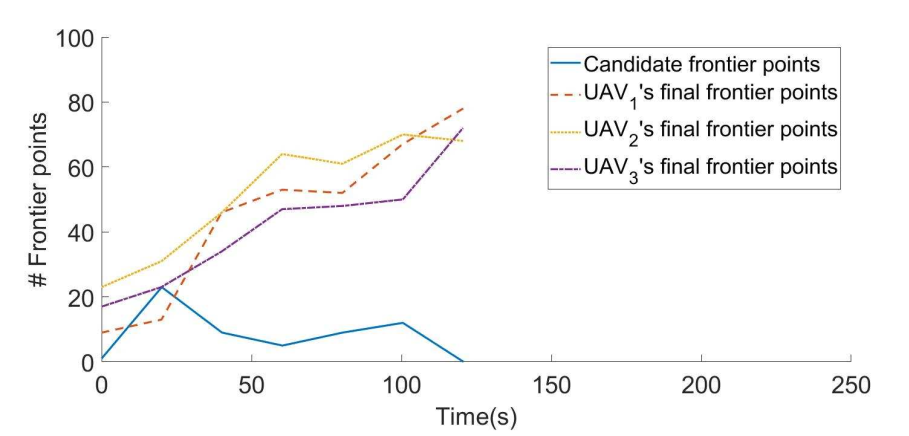
\includegraphics[chiều rộng=\linewidth]{assets/3_15_c.png}
        \caption{{Ba UAV kết hợp}}
        \label{fig:3.15c}
    \end{subfigure}
    \caption{Sự phát triển của ứng cử viên và số điểm biên giới cuối cùng trong quá trình thăm dò hợp tác.}
    \label{fig:3.15}
\end{figure}
\begin{figure}[H]
    \centering
    \begin{subfigure}[H]{0.5\linewidth}
        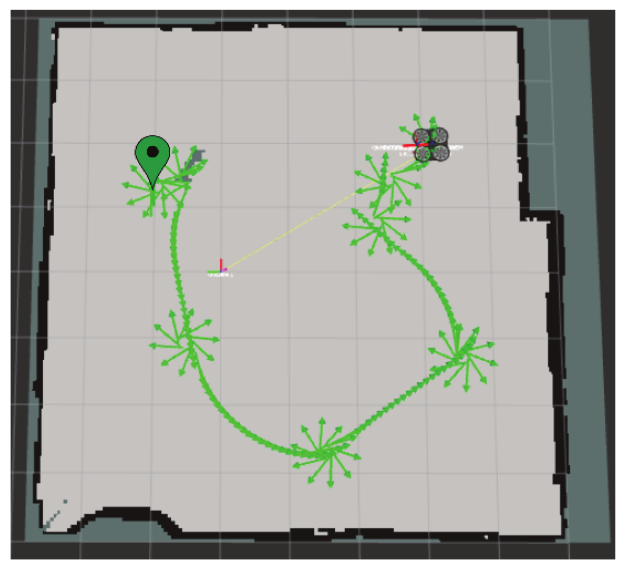
\includegraphics[chiều rộng=\linewidth]{assets/3_16_a.png}
        \caption{{Một UAV.}}
        \label{fig:3.16a}
    \end{subfigure}
    \begin{subfigure}[H]{0.5\linewidth}
        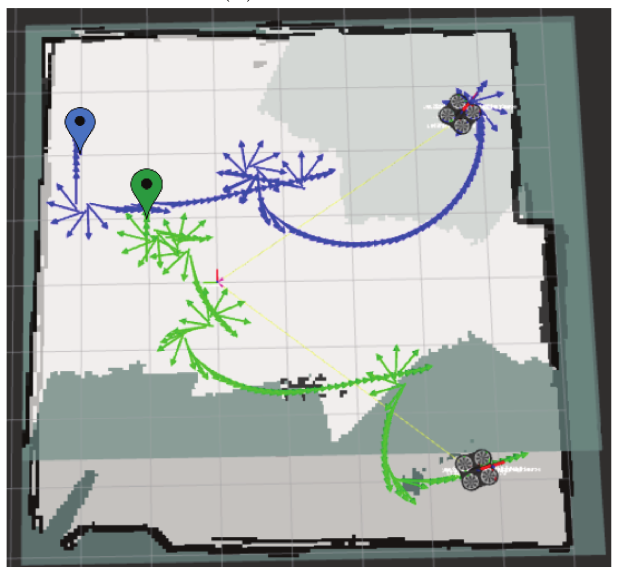
\includegraphics[chiều rộng=\linewidth]{assets/3_16_b.png}
        \caption{{Hai UAV hợp tác.}}
        \label{fig:3.16b}
    \end{subfigure}
    \begin{subfigure}[H]{0.5\linewidth}
        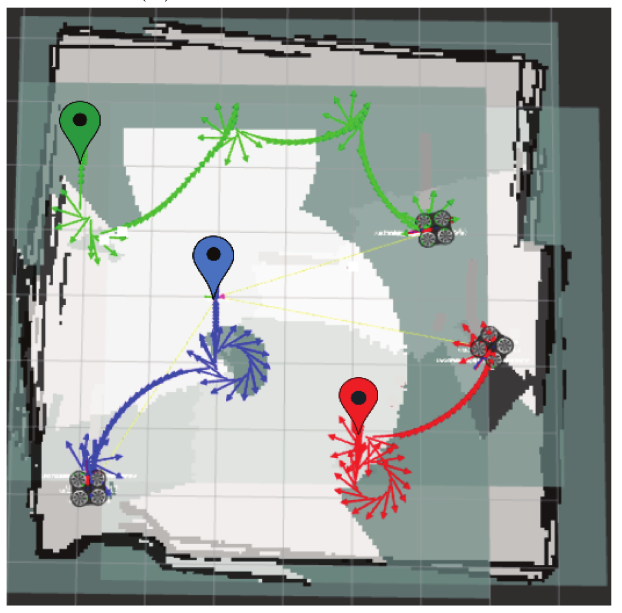
\includegraphics[chiều rộng=\linewidth]{assets/3_16_c.png}
        \caption{{Ba UAV hợp tác}}
        \label{fig:3.16c}
    \end{subfigure}
    \caption{Dự kiến bản đồ 2D trong một cuộc thám hiểm phối hợp với một nhóm một, hai và ba UAV.Các dấu hiệu và mũi tên màu xanh lá cây, xanh dương và đỏ xác định, tương ứng, vị trí ban đầu và quỹ đạo của UAV1, UAV2 và UAV3.}
    \label{fig:3.16}
\end{figure}
\subsubsection{Đánh giá nhiệm vụ mục tiêu: Phân phối robot trong môi trường}
Quá trình phân công mục tiêu được thực hiện theo thuật toán được mô tả trong Phần 3.6.Tuy nhiên, sau khi chỉ định mục tiêu cho robot đầu tiên trong danh sách, cùng một mục tiêu hoặc một mục tiêu khác gần với nó có thể được gán cho robot thứ hai trong danh sách.Để khắc phục những vấn đề này, mức tăng thông tin của các mục tiêu ứng cử viên còn lại được lên lịch.Điều này cho phép loại bỏ một mục tiêu đã được chỉ định và giữ một khoảng cách nhất định giữa mục tiêu mới và phần trước được chỉ định.\\\\
Giả sử rằng một mục tiêu được gán cho robot đầu tiên trong danh sách cụm.Hình \ref{fig:3.17} Hiển thị mục tiêu được chọn cho robot thứ hai khi một bài tập tuần tự được thực hiện:
\begin{itemize}
    \item Không cần xử lý điểm biên giới hơn nữa (xem hình \ref{fig:3.17b}). Do đó, mục tiêu tương tự được gán cho hai robot khác nhau.
    \item Trong khi loại bỏ mục tiêu được gán từ các điểm biên giới ứng cử viên còn lại (xem Hình \ref{fig:3.17c}). Do đó, mục tiêu thứ hai tương đối gần với người đầu tiên được chỉ định.
    \item Trong khi lên lịch trình thông tin tăng sau mỗi lần gán mục tiêu (xem Hình \ref{fig:3.17d}). Do đó, các mục tiêu được chỉ định được cách nhau vào môi trường.Lợi ích thông tin được lên lịch theo lịch trình Eq. \ref{eq:3.5}. Giá trị thông tin tăng lên với khoảng cách đến mục tiêu ứng viên $\mathbf{t}_g$.
\end{itemize}
Quá trình phân công mục tiêu đôi khi có thể không tối ưu vì nó phụ thuộc vào thứ tự của robot trong danh sách.Ví dụ, giả sử robot UAV$_i$ và UAV$_j$ có cùng một nhiệm vụ mục tiêu tốt nhất t k sao cho nó đạt được tiện ích tối đa so với các điểm biên giới ứng viên, nơi Eq.\ref{eq:3.6} và Eq. \ref{eq:3.7} được xác minh.
\begin{equation}\label{eq:3.6}
    \mathbf{t}_k=argmax_{t_m}\mathbf{U}(UAV_i,\mathbf{t}_m)
\end{equation}
với $\mathbf{t}_m \in \mathcal{G}$.
\begin{equation}\label{eq:3.7}
    \mathbf{t}_k=argmax_{t_n}\mathbf{U}(UAV_j, \mathbf{t}_n)
\end{equation}
với $\mathbf{t}_n \in \mathcal{G}$.\\
UAV$_i$ có một điểm biên giới ứng cử viên khác $\mathbf{t}_l$ với:
\begin{equation}\label{eq:3.8}
    \mathbf{\mathit{U}}(UAV_i, \mathbf{t}_k) > \mathbf{\mathit{U}}(UAV_i,\mathbf{t}_l) > \mathbf{\mathit{U}}(UAV_j, \mathbf{t}_k)
\end{equation}

\begin{figure}[H]
    \centering
    \begin{subfigure}[H]{0.6\linewidth}
        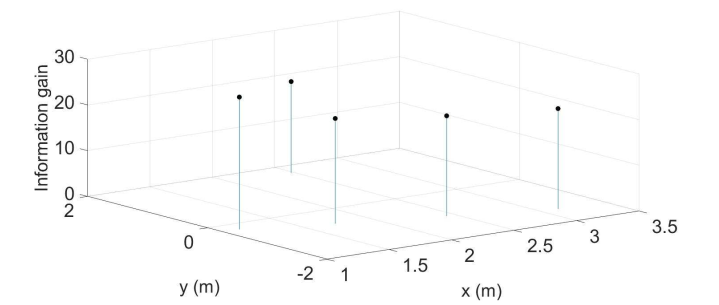
\includegraphics[chiều rộng=\linewidth]{assets/3_17_a.png}
        \caption{{Mục tiêu ứng viên.}}
        \label{fig:3.17a}
    \end{subfigure}
    \begin{subfigure}[H]{0.6\linewidth}
        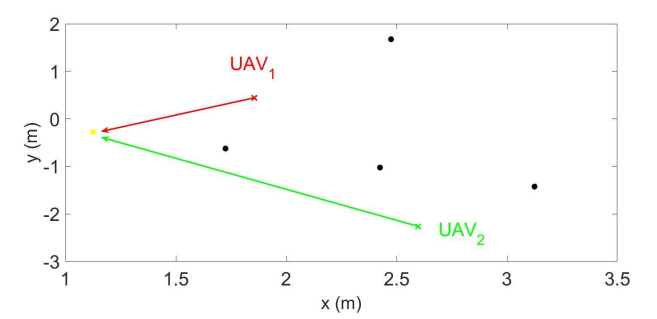
\includegraphics[chiều rộng=\linewidth]{assets/3_17_b.png}
        \caption{{Trường hợp 1.}}
        \label{fig:3.17b}
    \end{subfigure}
    \begin{subfigure}[H]{0.6\linewidth}
        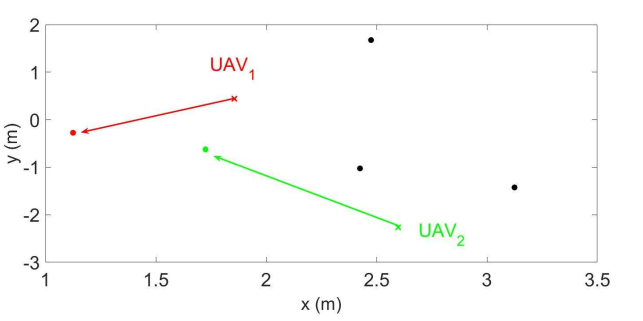
\includegraphics[chiều rộng=\linewidth]{assets/3_17_c.png}
        \caption{{Trường hợp 2.}}
        \label{fig:3.17c}
    \end{subfigure}
    \begin{subfigure}[H]{0.6\linewidth}
        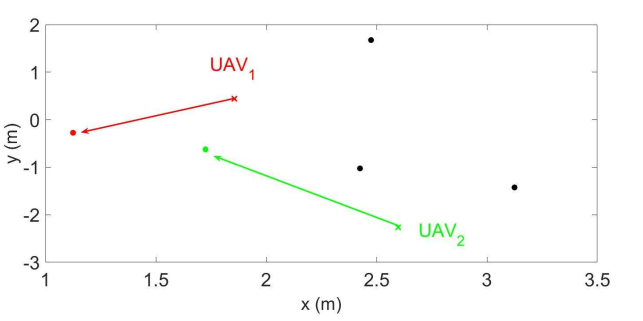
\includegraphics[chiều rộng=\linewidth]{assets/3_17_c.png}
        \caption{{Trường hợp 3.}}
        \label{fig:3.17d}
    \end{subfigure}
    \caption{Nhiệm vụ mục tiêu: Sau khi chỉ định một mục tiêu để UAV$_1$ , Một mục tiêu được chỉ định theo cách liên tiếp để UAV$_2$ . (a) đại diện cho các điểm biên giới ứng cử viên với mức tăng thông tin tương ứng của họ.(b), (c) và (d) đại diện, tương ứng, nhập mục tiêu khi: Không có quy trình nào khác được thực hiện cho các mục tiêu ứng cử viên còn lại; UAV$_1$ ’s Mục tiêu được loại bỏ khỏi các mục tiêu ứng cử viên còn lại và;Việc đạt được thông tin của các mục tiêu ứng cử viên còn lại được lên lịch.}
    \label{fig:3.17}
\end{figure}
Vì vậy, giải pháp tối ưu sẽ là gán $\mathbf{t}_l$ đến UAV$_i$ và $\mathbf{t}_k$ đến UAV$_j$ . Nhưng nếu UAV$_i$ là đầu tiên trong danh sách, $\mathbf{t}_k$ được gán cho nó và một điểm biên lai khác với ít tiện ích hơn $\mathbf{t}_k$, được chỉ định cho UAV$_j$. Do đó, giải pháp với việc phân công mục tiêu tuần tự không phải lúc nào cũng tối ưu.\\\\
Để khắc phục vấn đề này, tất cả các số kết hợp có thể xảy ra $\frac{n_g!}{n_g!(n_g-n_c)!}$ với $n_g$ số lượng mục tiêu ứng cử viên và $n_c$ số lượng robot, cần phải được xem xét.Điều này tăng đáng kể thời gian tính toán bằng cách tăng số lượng robot.Do đó, trong thuật toán được đề xuất, nhiệm vụ tuần tự được ưa chuộng về việc tính toán tất cả các hoán vị có thể.
\subsubsection{Khám phá đánh giá tỷ lệ không gian}
Đánh giá này nhằm định lượng lượng không gian khám phá trong nhiệm vụ. Hình \ref{fig:3.18} cho thấy tỷ lệ không gian được khám phá được thực hiện bởi mỗi UAV trong FL EET.Càng nhiều UAV trong môi trường, tỷ lệ thăm dò càng ít yêu cầu.Một robot không cần phải tiếp tục khám phá một khu vực nếu nó đã được khám phá bởi một khu vực khác.Do đó, thời gian nhiệm vụ giảm đáng kể.
\subsubsection{Đánh giá tỷ lệ chồng chéo}
Việc sử dụng một quy trình phân công mục tiêu artective e ff sẽ giới hạn sự chồng chéo được tạo. Trong hình \ref{fig:3.19}, Sự phát triển thời gian của sự chồng chéo được đánh giá bằng hai robot hợp tác.Sự chồng chéo trải qua một sự gia tăng đáng kể vào cuối cuộc thám hiểm để đạt được $33\%$. Điều này được giải thích bởi sự gần gũi của các bản đồ địa phương vào cuối nhiệm vụ chính xác là bản đồ lưới toàn cầu.
\begin{figure}[H]
    \centering
    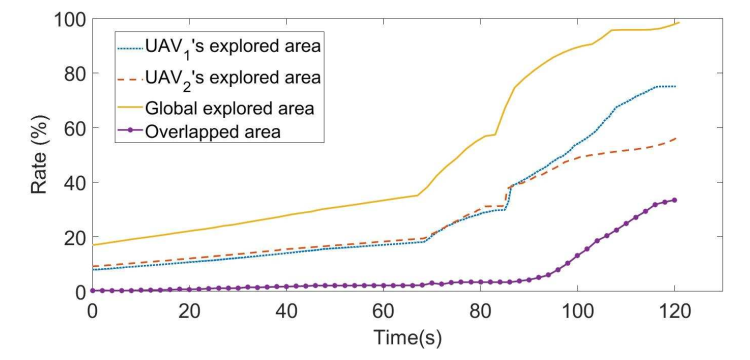
\includegraphics[tỉ lệ=0.4]{assets/3_19.png}
    \caption{Tỷ lệ khu vực khám phá và chồng chéo bằng cách sử dụng hai UAV hợp tác.}
    \label{fig:3.19}
\end{figure}
\subsubsection{Đánh giá khoảng cách di chuyển}
Đến e ff đánh giá ectively đánh giá hiệu suất chiến lược thăm dò về khoảng cách di chuyển của mỗi UAV, di ff erent chạy với một, hai và ba UAV đã được tiến hành trong đó tỷ lệ khu vực được khám phá gần như $99\%$. Hình \ref{fig:3.20} cho thấy khoảng cách được di chuyển bởi mỗi UAV trong FL EET trong nhiệm vụ.
\begin{figure}[H]
    \centering
    \begin{subfigure}[H]{0.7\linewidth}
        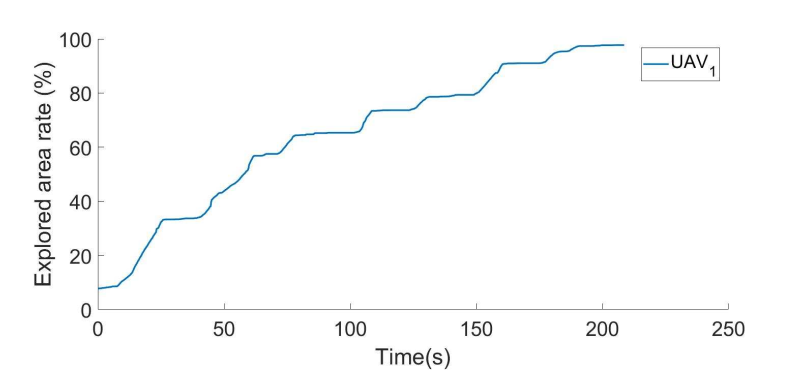
\includegraphics[chiều rộng=\linewidth]{assets/3_18_a.png}
        \caption{{Một UAV.}}
        \label{fig:3.18a}
    \end{subfigure}
    \begin{subfigure}[H]{0.7\linewidth}
        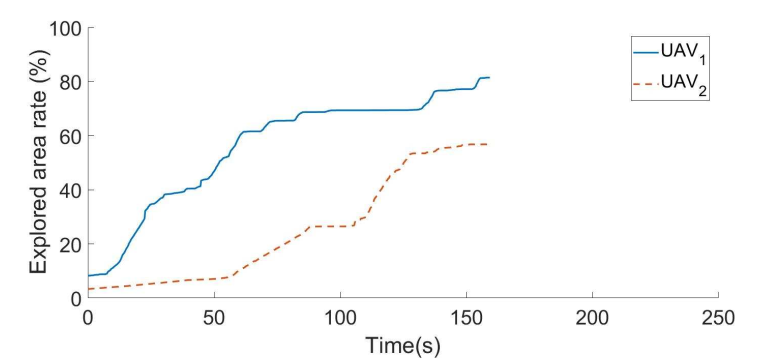
\includegraphics[chiều rộng=\linewidth]{assets/3_18_b.png}
        \caption{{Hai UAV hợp tác.}}
        \label{fig:3.18b}
    \end{subfigure}
    \begin{subfigure}[H]{0.7\linewidth}
        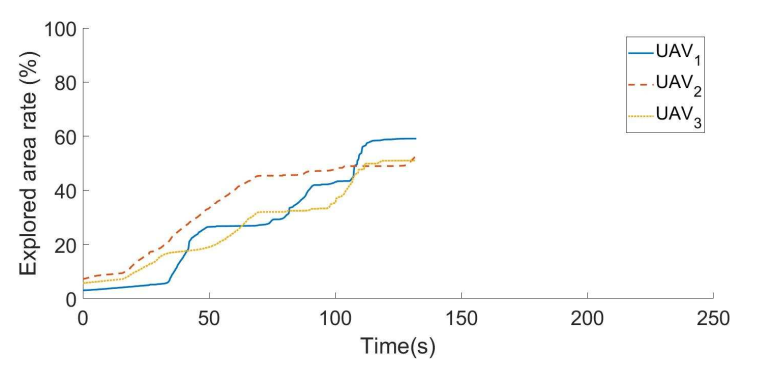
\includegraphics[chiều rộng=\linewidth]{assets/3_18_c.png}
        \caption{{Ba UAV hợp tác}}
        \label{fig:3.18c}
    \end{subfigure}
    \caption{Khám phá tỷ lệ không gian với một, hai và ba UAV.}
    \label{fig:3.18}
\end{figure}
\begin{figure}[H]
    \centering
    \begin{subfigure}[H]{0.7\linewidth}
        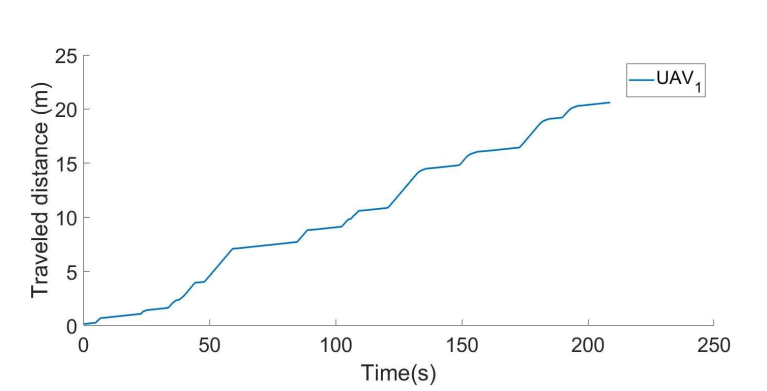
\includegraphics[chiều rộng=\linewidth]{assets/3_20_a.png}
        \caption{{Một UAV.}}
        \label{fig:3.20a}
    \end{subfigure}
    \begin{subfigure}[H]{0.7\linewidth}
        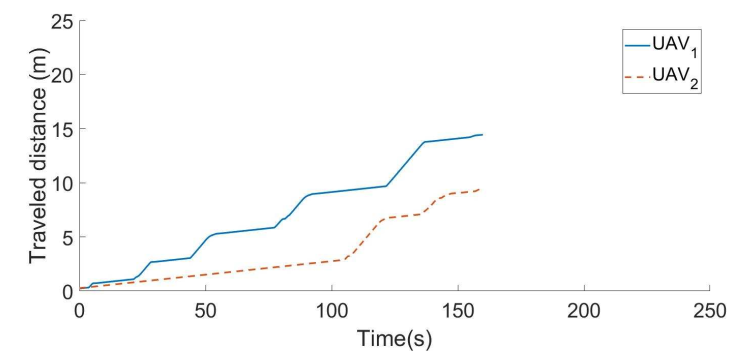
\includegraphics[chiều rộng=\linewidth]{assets/3_20_b.png}
        \caption{{Hai UAV hợp tác.}}
        \label{fig:3.20b}
    \end{subfigure}
    \begin{subfigure}[H]{0.7\linewidth}
        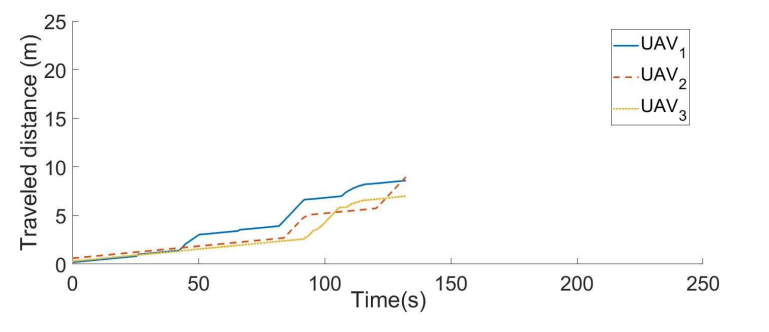
\includegraphics[chiều rộng=\linewidth]{assets/3_20_c.png}
        \caption{{Ba UAV hợp tác}}
        \label{fig:3.20c}
    \end{subfigure}
    \caption{Di chuyển khoảng cách bằng mỗi UAV với một, hai và ba UAV hợp tác.}
    \label{fig:3.20}
\end{figure}
Các khoảng cách được di chuyển bởi mỗi UAV bằng cách sử dụng một, hai và ba UAV trong FL EET được so sánh trong hình \ref{fig:3.21}. Khoảng cách này giảm với số lượng UAV.Khoảng cách trung bình được di chuyển bởi mỗi UAV bị giảm bởi $55\%$ cho 2 UAV và bởi $62\%$ cho 3 UAV.Lỗi của khoảng cách di chuyển được giảm nhẹ từ một đến hai và ba UAV.
\begin{figure}[H]
    \centering
    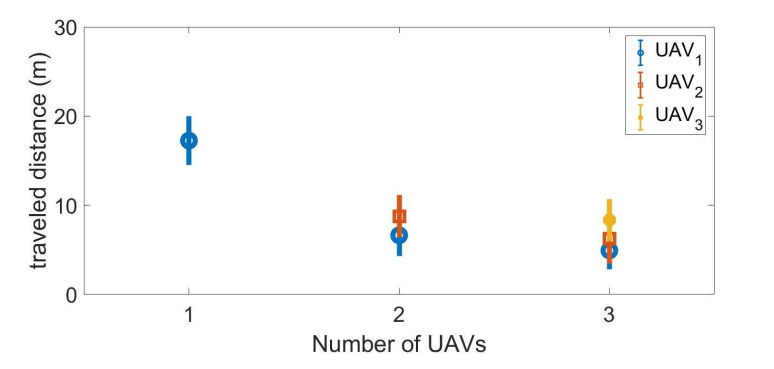
\includegraphics[scale=0.4]{assets/3_21.png}
    \caption{Đi du lịch đánh giá khoảng cách.}
    \label{fig:3.21}
\end{figure}
\subsubsection{Đánh giá thời gian khám phá}
Đối với đánh giá thời gian thăm dò, di ff erent chạy đã được thực hiện bằng cách sử dụng UAV 1, 2 và 3. Hình \ref{fig:3.22} Cho thấy rằng trung bình của thời gian thăm dò giảm khi số lượng robot trong EET tăng.Lỗi tính toán cũng giảm.Thời gian bị giảm bởi $25\%$ cho 2 UAV và bởi $30\%$ cho 3 UAV. Thời gian và khoảng cách thăm dò không được chia cho 2 hoặc 3 khi nhân với 2 hoặc 3 số lượng robot, tương ứng.Trong các mô phỏng này, vị trí ban đầu của robot là: $(1,0,0)$ cho một UAV; $(1,0,0)$ và $(1,-3,0)$ cho hai UAV;và $(1,1,0)$, $(1,-1,0)$ và $(1,-3,0)$ cho ba UAV.
\begin{figure}[H]
    \centering
    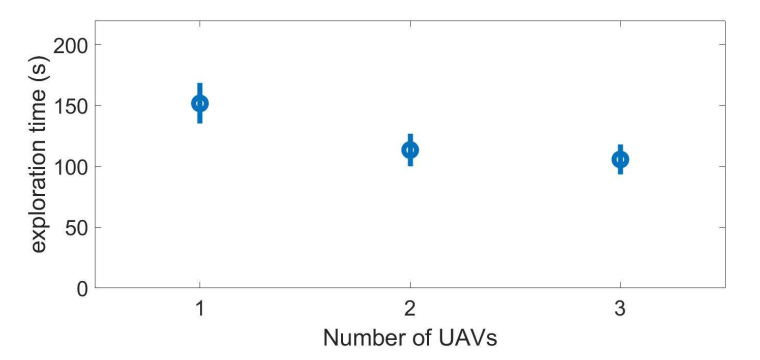
\includegraphics[tỉ lệ=0.4]{assets/3_22.png}
    \caption{Thời gian thăm dò trung bình.}
    \label{fig:3.22}
\end{figure}
Các kết quả được trình bày trong Phần 4.2 được đánh giá mà không có bản địa hóa tương đối.Vì vậy, để có một kịch bản thực tế khó khăn hơn, chạy với thuật toán bản địa hóa tương đối đã được thực hiện để đánh giá các màn trình diễn hệ thống bằng SLAM.
\subsection{Nhiệm vụ khám phá bằng thuật toán bản địa hóa tương đối}
Hướng tới một kịch bản thực tế hơn, cách tiếp cận ORB-SLAM2 (được giới thiệu trong Phần 5 của Chương 2) đã được triển khai để thực hiện bản địa hóa tương đối (xem Hình \ref{fig:3.23}).
\begin{figure}[H]
    \centering
    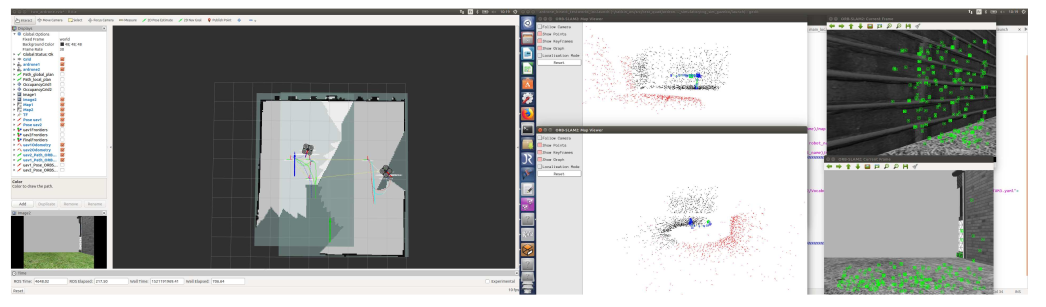
\includegraphics[tỉ lệ=0.3]{assets/3_23.png}
    \caption{Hai điều hướng UAV bằng ORB-SLAM2.Hình ảnh Rviz (trái) hiển thị, đối với mỗi UAV, bản đồ lưới chiếm dụng 2D được xây dựng, quỹ đạo ước tính và sự thật tương ứng.Đám mây điểm (giữa) đại diện cho việc tái thiết thưa thớt môi trường được thực hiện bởi mỗi UAV.Và, các điểm đánh dấu màu xanh lá cây (phải) đại diện cho các tính năng được tính bằng mỗi UAV để thực hiện bản địa hóa.}
    \label{fig:3.23}
\end{figure}
Mỗi robot thực hiện Slam nơi nó xây dựng bản đồ của nó trong khung tham chiếu cục bộ của nó $^WF_i$ , và ước tính tư thế tương đối của nó $\mathbf{p}_i$ bên trong nó. Sau đó, thiết bị thực hiện khám phá hợp tác bằng cách sử dụng một số thông tin cụ thể được trao đổi giữa các UAV. Tuy nhiên, những thông tin này phải nằm trong một hệ quy chiếu chung. Do đó, những thông tin như tư thế $\mathbf{p}_i$ và các điểm biên cương $\mathbf{f}_{i,j}$ nhất thiết phải biến thành khung tham chiếu toàn cầu $^0W$ trước khi được trao đổi.Vì thế \textit{leader} làm cho tất cả các tính toán cần thiết và gửi lại cho \textit{explorers} các mục tiêu trong $^0W$. Khi robot nhận được mục tiêu được giao, nó sẽ biến nó thành $^WF_i$ để lên kế hoạch cho một con đường đến nó.\\\\
Để thực hiện một phép chuyển đổi từ tham chiếu cục bộ $^WF_i$ đến toàn cầu một. $^0W$, Robot phải biết - ít nhất là - tư thế ban đầu của nó w.r.t. $^0W$. Như được giải thích trong Phần 5.2 của Chương 1, khung tham chiếu toàn cầu của môi trường được khởi tạo sao cho nó trùng với khung tham chiếu cục bộ của nhóm RST-\textit{leader} trong đội đó là UAV$_1$ Trong ví dụ được coi là phương trình \ref{eq:3.9}.
\begin{equation}\label{eq:3.9}
    ^0W\equiv ^WF_1,
\end{equation}
Sau đó, bằng cách phát hiện robot này bằng các thẻ được gắn trên đó, các robot khác có thể ước tính biến đổi tương ứng của chúng thành nó $^{F_j}\begin{bmatrix}\mathbf{R} & \mathbf{t}\end{bmatrix}_{F_1}, j \in [2..n_c]$. Để đánh giá mô phỏng, thông tin về biến đổi - được tính toán trong khi phát hiện thẻ - được giả định sẽ được biết đến. Hình \ref{fig:3.24} Cho thấy sự phát triển tỷ lệ thăm dò trong nhiệm vụ thăm dò trong khi sử dụng ORB-SLAM2 làm phương pháp nội địa hóa tương đối.Thời gian truyền bá sử dụng ORB-SLAM2 bị giảm bởi $43\%$ Đối với 2 UAV thay vì 1 UAV.
\begin{figure}[H]
    \centering
    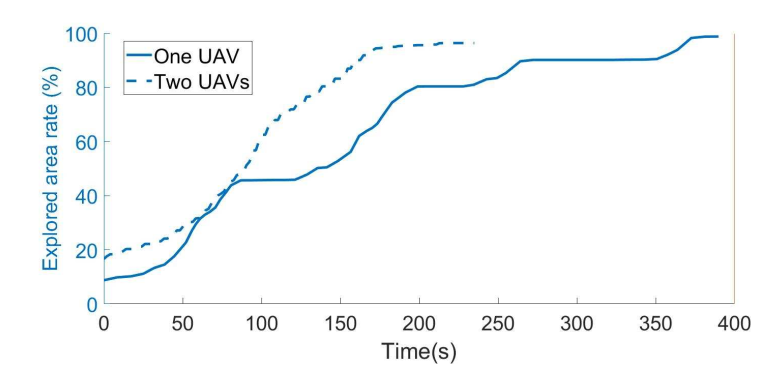
\includegraphics[tỉ lệ=0.4]{assets/3_24.png}
    \caption{Khám phá sự tiến hóa tỷ lệ khu vực trong nhiệm vụ thăm dò với một và hai UAV trong khi thực hiện ORB-SLAM2 bởi mỗi UAV.}
    \label{fig:3.24}
\end{figure}
Thời gian thăm dò khi sử dụng bản địa hóa tương đối (xem hình \ref{fig:3.24}) tương đối quan trọng so với việc khám phá mà không có slam (xem hình \ref{fig:3.18}) Vì vận tốc đã giảm đáng kể.
\section{Phần kết luận}
Trong chương này, chúng tôi đã trình bày một trạng thái của nhiệm vụ thăm dò đa robot bao gồm chiến lược được sử dụng để chỉ định robot cho mục tiêu và một chức năng tiện ích được áp dụng để ước tính sự quan tâm của việc tiếp cận nó.Sau đó, chúng tôi đã giới thiệu một chiến lược thăm dò dựa trên nhóm-\textit{leader} quyết định. Bài tập robot-mục tiêu được thực hiện bằng cách sử dụng chức năng tiện ích mới lạ.Hàm này tạo ra một giao dịch giao dịch giữa khám phá nhanh và nhận bản đồ lưới chi tiết, và cũng có tính đến khoảng cách của mỗi robot trong nhóm từ bộ mục tiêu chưa được khám phá.Ngoài ra, chúng tôi đề xuất để lên lịch để đạt được thông tin để e FFI tiêu hóa tiêu hóa UAV vào môi trường.Hơn nữa, chiến lược được thông qua trao đổi các điểm biên giới thay vì toàn bộ bản đồ địa phương.\\\\
Kết quả cho thấy chiến lược thăm dò hợp tác đề xuất giảm thiểu thời gian thăm dò toàn cầu theo $25\%$ cho 2 UAV và bởi $30\%$ cho 3 UAV, đồng thời giảm thiểu khoảng cách trung bình di chuyển của mỗi UAV bởi $55\%$ cho 2 UAV và bởi $62\%$ cho 3 UAV.Hơn nữa, chiến lược được đánh giá bằng thuật toán nội địa hóa tương đối nơi giảm thời gian thăm dò $43\%$ Đối với 2 UAV thay vì 1 UAV.
%------------------CHAPTER 4------------------------------------------------%
\chapter{Giao tiếp giữa các robot}
\section{Giới thiệu}
Một chủ đề quan trọng trong các hệ thống nhiều robot là giao tiếp giữa các robot. Tính năng này được sử dụng để điều phối và chia sẻ thông tin cụ thể. Một đội có thể được triển khai trong một số nhiệm vụ trong các khu vực tương đối khác biệt và thù địch. Tuy nhiên, những môi trường này có thể không có cơ sở hạ tầng mạng sẵn có, ngoài các liên kết truyền thông không lý tưởng.\\\\
% This chapter highlights one of the most challenging points in MRS, which is the inter- robot communication. This problem can be addressed from different perspectives; but, we have chosen to study two sub-problems, which are: network typology, and network topology and strategy for MRS robustness.
Chương này nhấn mạnh một trong những điểm thách thức nhất trong MRS, đó là giao tiếp giữa các robot. Vấn đề này có thể được giải quyết từ các quan điểm khác nhau; nhưng, chúng tôi đã lựa chọn nghiên cứu hai vấn đề nhỏ, đó là: định dạng mạng, cấu trúc liên kết mạng và chiến lược cho sự mạnh mẽ của MRS.
\section{Phân loại mạng}
% The network is used to link between different entities and to establish possible communi- cation between them. Several network types exist and can be classified in different ways.
Mạng được sử dụng để liên kết giữa các thực thể khác nhau và để thiết lập giao tiếp có thể có giữa chúng. Một số loại mạng tồn tại và có thể được phân loại theo nhiều cách khác nhau.
\subsection{Chế độ cơ sở hạ tầng so với chế độ không có cơ sở hạ tầng}
Để quản lý cơ sở hạ tầng mạng, các chế độ hiện có có thể được phân loại thành hai loại chính \cite{bekmezci2013flying},\cite{hayat2015experimental}. Loại đầu tiên là chế độ cơ sở hạ tầng, có thể được gọi là chế độ Điểm truy cập (AP) và loại thứ hai là chế độ không có cơ sở hạ tầng, gọi là Ad Hoc mode (Xem Hình \ref{fig:4.1}). Trong chế độ AP, giao tiếp UAV-to-UAV được thực hiện thông qua cơ sở hạ tầng (AP, bộ định tuyến, v.v.), không giống như chế độ Ad Hoc trong đó các nút giao tiếp trực tiếp với nhau. Chế độ Ad Hoc còn được gọi là chế độ ngang hàng. Mạng Ad Hoc có thể phát triển thành một chế độ ngang hàng khác được gọi là mạng lưới bằng cách cho phép khả năng đa bước. Thật vậy, mạng Ad-Hoc không có bất kỳ khả năng cố hữu nào cho đa bước. Các nút giao tiếp với nhau khi chúng nằm trong phạm vi giao tiếp của nhau. Trong khi đó, trong mạng lưới, các nút có thể giao tiếp trực tiếp hoặc thông qua một hoặc nhiều nút trung gian.
\begin{figure}[H]
    \centering
    \includegraphics[scale=0.4]{assets/4_1.png}
    \caption{Chế độ hạ tầng (trái) và chế độ không có hạ tầng (phải).}
    \label{fig:4.1}
\end{figure}
\begin{table}[H]
    \centering
    \caption{Chế độ cơ sở hạ tầng so với chế độ không có cơ sở hạ tầng.}
    \label{tab:4.1}
    \begin{tabular}{|l|p{4.5cm}|p{4.5cm}|}\hline
                            & \textbf{Chế độ cơ sở hạ tầng}                 & \textbf{Chế độ không có cơ sở hạ tầng}
        \\\hline
        \textbf{Ưu điểm}    & Giao tiếp đáng tin cậy                        & Kết nối trực tiếp với nhau, dễ thiết lập, mạnh mẽ với lỗi nút, cho phép mở rộng và điều chỉnh trong cấu trúc liên kết mạng. \\\hline
        \textbf{Nhược điểm} & Phần cứng đắt, phức tạp, phạm vị bị hạn chế . & Thừa trong kết nối mạng, khó bảo trì.                                                                                       \\\hline
        \textbf{Tiêu chuẩn} & 802.11                                        & 802.11, 802.15, 802.16                                                                                                      \\\hline
    \end{tabular}
\end{table}
Ban đầu, robot phải thực hiện nhiệm vụ của chúng trong môi trường không có cơ sở hạ tầng mạng. Trên thực tế, chúng trao đổi thông tin khi chúng hoạt động như một bộ định tuyến và như một AP. Vì vậy, hệ thống MRS có thể được xem như một mạng Ad Hoc di động theo quan điểm giao tiếp.
\subsection{Phân loại mạng Ad Hoc}
Mạng Ad Hoc là mạng được sử dụng phổ biến để quản lý giao tiếp đa robot. Với mạng này, mỗi robot có thể di chuyển tự do và chuyển tiếp các gói tin đến và từ mỗi robot khác tùy thuộc vào phương thức phân phối dữ liệu \cite{bouachir2014conception}. Mạng này được đặc trưng bởi chất lượng dịch vụ phức tạp, trong đó giao thức định tuyến xác định đường đi tối ưu của thông tin có tính đến sự thay đổi thường xuyên của cấu trúc liên kết. Thêm vào đó, sẽ rẻ hơn nếu nhận ra loại mạng này thay vì các loại khác (vệ tinh, di động, v.v.).\\\\
Mạng Ad Hoc có thể được phân loại thành ba loại chính là Mobile Ah doc NETwork (MANET), Vehicle Ah doc NETwork (VANET) và Flying Ad hoc NETworks (FANET). Nói chung, đối với hệ thống đa UAV, mô hình FANET được sử dụng. Bảng \ref{tab:4.2} mô tả chi tiết mỗi đặc điểm của danh mục \cite{bekmezci2013flying}, \cite{maistrenko2016experimental}, phân tích dự đoán của chúng tôi.
\begin{table}[H]
    \centering
    \caption{So sánh giữa MANET, VANET, FANET và mô hình mạng của chúng tôi.}
    \label{tab:4.2}
    \begin{tabular}{|p{2.8cm}|p{1.5cm}|p{1.5cm}|p{1.8cm}|p{1.8cm}|}\hline
        \textbf{Đặc điểm}                                                 & \textbf{MANET}                                      & \textbf{VANET}                       & \textbf{FANET}                                                                                 & \textbf{Mô hình mạng của chúng tôi}
        \\\hline
        \textbf{Tính di động}                                             & Người ở một số địa hình nhất định                   & Phương tiện ở cao tốc                & Máy bay trong kế hoạch 3D                                                                      & 3D                                  \\\hline
        \textbf{Mức độ di động}                                           & $+$                                                 & $+$                                  & $++$                                                                                           & $++$                                \\\hline
        \textbf{Chế độ di động}                                           & Điểm cách ngẫu nhiên với hướng và tốc độ ngẫu nhiên & Có khả năng dự đoán cao trên đường   & Không được xác định trước (mô hình chuyển động ngẫu nhiên của UAV, mô hình dựa trên pheromone) & Có thể dự đoán                      \\\hline
        \textbf{Thay đổi cấu trúc liên kết}                               & $+$                                                 & $+$                                  & $++$                                                                                           & $++$                                \\\hline
        \textbf{Khoảng cách giữa các nút}                                 & $+$                                                 & $+$                                  & $++$                                                                                           & $+$                                 \\\hline
        \textbf{Mật độ nút}                                               & $++$                                                & $++$                                 & $+$                                                                                            & $+$                                 \\\hline
        \textbf{Mô hình truyền thanh}                                     & Sự hiện diện hiếm hoi của đường ngắm                & Sự hiện diện hiếm hoi của đường ngắm & Sự hiện diện thường xuyên của đường ngắm                                                       & Luôn có mặt của đường ngắm          \\\hline
        \textbf{Công suất tiêu thụ và công suất tính toán thời gian sống} & $+$                                                 & $+$                                  & $++$                                                                                           & $++$                                \\\hline
        \textbf{Tiêu chuẩn}                                               & IEEE 802.11, 802.15, 802.15.4, 802.16 and 802.20    & IEEE 802.11p                         & IEEE 802.11                                                                                    & ?                                   \\\hline
    \end{tabular}
\end{table}
So sánh cho thấy FANET là mạng gần nhất với kỳ vọng của mô hình của chúng tôi. Do đó, trong số các tiêu chuẩn hiện có cho loại mạng này, IEEE 802.11b và IEEE 802.11g cung cấp tốc độ dữ liệu cao và thường được sử dụng cho các hệ thống nhiều robot.
\subsection{Phân loại cấu trúc liên kết mạng}
Cấu trúc liên kết mạng xác định điểm đầu, điểm cuối và đường dẫn của thông tin trong mạng. Đã cho các điểm mục tiêu, cấu trúc liên kết xác định tất cả các con đường có thể để đạt được chúng.\\\\
Từ quan điểm phần mềm, mạng chủ yếu có thể được phân loại theo ba cấu trúc liên kết (Xem Hình \ref{fig:4.2}\footnote{Source: From user 1983 on Wikipedia. Licensed CC BY-SA}):
\begin{figure}[H]
    \centering
    \includegraphics[scale=0.4]{assets/4_2.png}
    \caption{Mạng tập trung (trái), phi tập trung (giữa) và mạng phân tán (phải).}
    \label{fig:4.2}
\end{figure}
\begin{itemize}
    \item Mạng tập trung: Đây là cấu trúc liên kết được sử dụng nhiều nhất \cite{morgenthaler2012uavnet}, \cite{forster2013collaborative}. Tất cả các nút - còn được gọi là các trạm - được kết nối với nhau thông qua một trung tâm tập trung. Đó là khi một nút cần gửi một thông tin đến một nút khác, dữ liệu nhất thiết phải đi qua nút trung tâm để được chuyển đến đích của nó. Nếu nút trung tâm không hoạt động hoặc không thể truy cập được, không có dữ liệu nào có thể được truyền đi, điều này làm cho cấu trúc liên kết này dễ bị lỗi nút.
    \item Decentralized network: This topology is considered as a set of centralized networks connected together \cite{konolige2003map}, \cite{brand2014stereo}. One central hub is employed for every little group of nodes to send and receive the information. If a hub fails, nodes which are direactly relied to it become inaccessible.
    \item Distributed network: This topology contains nodes that are connected to each others. Unlike the centralized topology, several paths are possible to reach one destination. Also, nodes are not affected by one node's failure. This allows to increase the survivability and to decrease the vulnerability of the network. The distributed topology is attractive to ensure reliable network \cite{cunningham2010ddf}. Nevertheless, it is quite difficult to reach and to realize in reality, and the simulation are not fully distributed \cite{waharte2009coordinated}, \cite{cameron2009collaborative}, \cite{scherer2015autonomous}. This is because all processing and decision making have to be on-board the robot whichs requires an important memory and a heavy computation.
\end{itemize}
\section{Network typology}
The typology of the network represents its type and, accordingly, the characteristics introduced.
\subsection{Related work}
MRS communication is a critical problem to tackle in the robotics community. In the last decade, the great progress in wireless technologies and MRS has created a growing interest for inter-robot communication. Hence, different methods have been proposed.\\\\
To face disaster scenarios such as fire in an industrial warehouse, authors in \cite{witkowski2008ad} propose to use Wireless LAN, Bluetooth and ZigBee to form an Ad- Hoc network. Some robots of the fleet form the network infrastructure to support communication.\\\\
Authors in \cite{morgenthaler2012uavnet} use two network standards to build a multi-UAV system. A IEEE 802.11s wireless mesh network is build using UAVs carrying mesh nodes directly connected to the flight electronics. Each of these mesh nodes acts as an AP in order to form an IEEE 802.11g.\\\\
A methodology that profiles the wireless links for Linux-based networked aerial vehicles is presented in \cite{kuschnig2012profiling.} The approach includes two options to collect link quality information and to monitor the 802.11 wireless interface.\\\\
An evaluation of the standard 802.11a used between an UAV and an AP is performed in \cite{kuschnig2012profiling}. Results show that the Received Signal Strength (RSS) for the downlink decreases with the distance to the AP but remains at an acceptable level as well as the throughput.\\\\
Knowing that the visible light spectrum is much wider than the Radio Frequency spectrum, it seems interesting to uptake Visible Light Communication (VLC) based on Light Emitting Diodes (LEDs). IEEE has developed the 802.15.7 standard for short range communication using visible light. Authors in \cite{wang2014openvlc} introduce a bidirectional communication using Open VLC. This solution hardware needs a Beagle Bone Black (BBB) board and a font transceiver that employs a single LED to both transmit and receive. The solution is implemented on Linux driver that communicates directly with the LED front-end and the Linux networking stack. The main idea to reuse the same LED for both Transmitting (TX mode) and Receiving Light signal (RX mode) is that when a node is transmitting data, the other node can expect the LOW symbol of the bit 0 and makes use of this time to switch his mode from RX to TX and transmit data.\\\\
The Zigbee – based on IEEE 802.15.4 – is a protocol of high level which is particularly useful for short communication range and low consumption. Several UAVs’ application use this network \cite{asadpour2014routing}. Communication can be made under three frequency bands depending on the chipset type: 868MHz for a bit rate of 20 kbps, 915MHz for 40 kbps and 2.4GHz for 250 kbps.\\\\
Authors in \cite{vidal2015multi} adopt different sized groups composed of tactical UAVs and UAVs moving in delimited geographical areas. Virtualization techniques are used to adapt the upgrade of any function, which allows the flexibility in heterogeneous services.\\\\
In a search and rescue mission, for example, authors in \cite{scherer2015autonomous} propose to do real-time streaming between UAVs over a large distance. The mission is divided into five principle phases: The pre-planning to define the best paths in the search area allowing to reduce the time of the mission then searching by just following the predefined way- points; the detection of the target and sending the new plans to the others, followed by the repositioning by setting a multi hop link to evaluate the situation by the base station and finally, the streaming of the video.\\\\
The multi-UAV, moving in a three dimensional space, need sophisticated transmission systems to ensure flexibility. In \cite{scherer2015autonomous}, an omni-directional isotropic antenna is fixed on the base station and on all the deployed heterogeneous UAVs. For data exchange, the standard IEEE 802.11s mesh technology is used.\\\\
Authors in \cite{hayat2015experimental} present a performances comparison between the stan- dard IEEE 802.11n and the IEEE 802.11ac in a multi hop network. Both networks were experimented in indoor and outdoor environment, and in two mode, the access point mode (AP)/infrastructure mode and the mesh mode regarding throughput and fairness. In indoor experiments, for an infrastructure mode, the 802.11ac shows improved performances in both TCP and UDP throughput, and packet loss for UDP traffic. In outdoor experiments, for infrastructure mode, the throughput of 802.11n is three time higher than that of 802.11a however, the link quality drops more steeply. For mesh mode, 802.11n achieves higher throughput at close range but drops faster as soon as date rate gets higher and the range longer. The recorded throughput for mesh network is lower than infrastructure mode due to the longer inter-packet transmission times.\\\\
To face issues of maintenance connectivity, collision avoidance, robustness to failure and area coverage improvement, authors in \cite{ghedini2018toward} propose a novel model that provides more efficient network topologies.\\\\
In \cite{harms2017development}, a new communication layer is proposed to deal with networks that requires a high bandwidth. For that, some mechanism are used to buffer messages, to compress data or to react to unexpected situations.\\\\
Table \ref{tab:4.3} lists some standards used in multi-robot systems. For each standard, we detail the concerned layer in the OSI model, its characteristics, the resulting performances, and the hardware and software used for experiments.
\begin{landscape}
    \begin{table}[H]
        \centering
        \caption{Examples of some standards used in MRS.}
        \label{tab:4.3}
        \begin{tabular}{|p{1.5cm}|p{1.7cm}|p{1.3cm}|p{2.9cm}|p{2.7cm}|p{2.3cm}|p{2cm}|}\hline
            \textbf{Work}                             & \textbf{Standard}            & \textbf{Layer}    & \textbf{Characteristics}                                                  & \textbf{Performances}                                                                    & \textbf{Hardware}                                                               & \textbf{Software}
            \\\hline
            [Scherer et al., 2015]                    & IEEE 802.11s mesh technology & Network layer     & Compatible with mesh mode and AP mode                                     & Range: 100m, communication delay: 5ms, Throughput: 10-20Mbit/s                           & Heterogeneous UAVs + laptop BS + wifi module                                    & Middleware Robot Operating System ROS       \\\hline
            \multirow{2}{1.5cm}{[Hayat et al., 2015]} & IEEE 802.11n                 & PHY and MAC layer & High throughput in both mode (AP and mesh), acceptable degree of fairness & Outdoor + mesh mode + single hop; Range: 500m; TCP throughput: 35Mbit/s (50m); FB: 40Mhz & Two Pelican UAVs + laptop BS + Compex WLE300NX 802.11abgn mini PCIe modules     & Ubuntu Linux Kernel 3.2. with ath9k driver  \\\cline{2-7}
                                                      & IEEE 802.11ac                & PHY and MAC layer & Do not support mesh mode                                                  & Outdoor + mesh mode + single hop; Range: 500m; TCP throughput: 10Mbit/s (50m); FB: 80Mhz & Two Pelican UAVs + laptop BS + Compex WLE900N518 802.11ac 5Ghz miniPCIe modules & Ubuntu Linux Kernel 3.2. with ath10k driver \\\hline
        \end{tabular}
    \end{table}
\end{landscape}
\begin{landscape}
    \begin{table}[H]
        \centering
        \begin{tabular}{|p{1.5cm}|p{1.7cm}|p{1.3cm}|p{2.9cm}|p{2.7cm}|p{2.3cm}|p{2cm}|}\hline
            [Kuschnig et al., 2012] & IEEE 802.11a           & PHY and MAC layer & RSS and throughput decreases with the distance but still at an acceptable level          & Outdoor over compus 150m*150m; Range: 10m; Throughput: 54Mbit/s (theo) and 27Mbit/s (prac); FB: 5Ghz                        & AP: Netgear WNDR3700 + Atheros AR9280 based wireless cards + UAV with Intel Atom Processor + SparkLAN WPEA110N wireless card + antenna WIMO 18720.11 for UAV and AP & Linux-based OpenWRT Backfire 10.03.1RC5 \\\hline
            [Asadpour et al., 2014] & IEEE 802.11n multi hop & PHY and MAC layer & Long convergence time and high routing overhead (with BATMAN protocol for Network Layer) & In-flight experiment; Throughput for 200m: 5.95Mbit/s; Convergence time (20-100m): 28s; Routing overhead (20-100m): 10msg/s & Two Arducopter + GB + WLAN IEEE 802.11n + XBEE-PRO                                                                                                                  &                                         \\\hline
        \end{tabular}
    \end{table}
\end{landscape}
\begin{landscape}
    \begin{table}[H]
        \centering
        \begin{tabular}{|p{1.5cm}|p{1.7cm}|p{1.3cm}|p{2.9cm}|p{2.7cm}|p{2.3cm}|p{2cm}|}\hline
            [Morgen- thaler et al., 2012] & IEEE 802.11s mesh nodes for UAV to UAV and IEEE 802.11g for UAV to AP & network layer     & In single hop, flying UAVs reach higher throughput than UAVs in the ground. These results are performed with the location based position mode which are lower than those with the signal strength positioning mode. These performances are higher than in multi-hop. & Single hop (1UAV altitude 3-5m and AP-AP = 75m) in location positioning mode; TCP throughput = 6.5Mbit/s + in signal strength positioning mode: TCP throughput = 8.1Mbit/s & One UAVNet quadcopters Professional Mesh OM1P + two notebooks & Linux 2.6.37.6 Kernel generated by ADAM (embedded Linux distribution) + driver ath5k \\\hline
            [Muzaffar and Yanmaz, 2014]   & IEEE 802.11ab                                                         & PHY and MAC layer & Throughput decreases with the increase of the number of nodes                                                                                                                                                                                                       & Range: up to $1000m \times 1000m \times 50m$; Throughput: 54Mbit/s (prac); FB: 5Ghz                                                                                        & Simulation: UAVs + Groung Station                             & Omnet++                                                                              \\\hline
        \end{tabular}
    \end{table}
\end{landscape}
\begin{landscape}
    \begin{table}[H]
        \centering
        \begin{tabular}{|p{1.5cm}|p{1.7cm}|p{1.3cm}|p{2.9cm}|p{2.7cm}|p{2.3cm}|p{2cm}|}\hline
            [Wang et al., 2014] & IEEE 802.15.7 & PHY and MAC layer & Bidirectional transmission, matching filtering and timing error recovery can increase the communication range and stability & \textit{One hop}: throughput: 1.6kb/s, packet loss ratio $5\%$; \textit{Two hop:} throughput 0.65kb/s, packet loss ratio $15\%$ & Embedded BBB board + LED front end & Linux Kernel 3.8.13 \\\hline
        \end{tabular}
    \end{table}
\end{landscape}
\subsection{Network standards and protocols}
Since the exchange of information is necessary for coordination, the network used for multi-UAV communication has to ensure that the information circulates properly throughout nodes. Consequently, we have to overcome some issues such as:
\begin{itemize}
    \item Node failure: When the link is broken or defected, the network must find a path to reach the node.
    \item Topology changes: Nodes move in the environment and generate changes in the topology that the network have to deal with rapidly.
    \item Communication bandwidth: UAVs possess certain information to exchange with other and need some bandwidth that supports the data exchange.
\end{itemize}
Taking into account the above cited issues, and to ensure agood integration between the visual SLAM and the communication, the distributed and cooperative wireless mesh network seems to be the most adequate network typology. It allows to introduce the following advantages:
\begin{itemize}
    \item Improving the network reliability because infrastructureless network offers several paths, so that information may reach the destination even if only one link is broken.
    \item Allowing self scalability of the network by a quick adaptation to topology changes.
    \item Enabling rapid deployment with lower cost back-haul.
    \item Providing easily coverage in areas which have difficult access.
    \item Saving battery life due to its lower power consumption.
    \item Enabling to face a growing number of UAVs in the fleet.
\end{itemize}
Among the existing mesh network standards, the 802.11s amendment, related to the MAC layer, is interesting for MRS applications. It is an Extended Service Set network that supports broadcast, multicast and unicast communication. It contains the Hybrid Wireless Mesh Protocol (HWMP) as the default routing protocol. The HWMP is a hybrid routing protocol inspired by the AODV (Ad-hoc On-demand Distance Vector: an on demand and reactive portion) and the tree based protocol (a proactive portion). Thereby, it contains the advantages of the reactive protocol since it prepares the routing table when nodes change their position, and thus provides the safer path. On the other hand, it contains the advantages of the proactive protocol since the routing table is ready which allow to save time when needed. In addition to the default routing protocol HWMP, the 802.11s mesh network supports other protocols like Optimized Link State Routing (OLSR), Better Approach to Mobile Ad hoc Networking (BATMAN), Wireless Distribution System (WDS), Open Shortest Path First (OSPF) and BABEL. According to \cite{wang2010experimental}, BATMAN proved better performances than HWMP and OLSR. Thus, experiments using HWMP and BATMAN have been performed to point out the saved data.
\paragraph{BATMAN protocol  definition}
The BATMAN\footnote{Source: \url{https://www.open-mesh.org/projects/open-mesh/wiki}} is a proactive routing protocol inspired by AODV and OLSR. It is supported by multi-hop Ad Hoc mesh networks. It uses different approaches to route selection node by periodically sending OriGinator Messages (OGM) to neighbors with node information to next hop and destination because the routing decisions are distributed on nodes. In this protocol, each node decides for the next hop and not for the whole route so nodes do not use or even know the topology of the network. In the case of detecting other nodes, BATMAN protocol finds the best route to them. It also keeps track of new nodes and informs its neighbors about their existence.
\subsection{Result and discussion}
For the evaluation of the networked system using BATMAN\footnote{The BATMAN-adv version used for the testbed is available since 2013} protocol, we use heteroge- neous nodes composed of three laptops: 2.40GHz dual core Linux machine, 2.27GHz i3 Linux machine, 2.50GHz i5 Linux machine and a Parrot AR-Drone 2.0 (See Figure \ref{fig:4.3}).
\begin{figure}[H]
    \centering
    \includegraphics[scale=0.3]{assets/4_3.png}
    \caption{Mesh network illustration between three laptops and one drone.}
    \label{fig:4.3}
\end{figure}
We simulate the broadcast of data between nodes in both Ad Hoc and mesh network with BATMAN protocol to underline the saved data. The drone was controlled from the laptop using a cross compilation. First, we perform an Ad Hoc network between endpoints and broadcast the data from node A to node B, C and D in the network. Then, we broadcast – in the same conditions – from node A to B, C and D with the BATMAN mesh network protocol. Results in Figure \ref{fig:4.4} show that the throughput achieved an average of 0.4 Mbits/s; whereas, the throughput evaluated in mesh network with BATMAN protocol, achieved an average of 0.65 Mbits/s. The BATMAN mesh network protocol improves by 1,5 times the throughput of the network compared to a basic Ad Hoc network.
\begin{figure}[H]
    \centering
    \includegraphics[scale=0.4]{assets/4_4.png}
    \caption{Broadcast testbed throughput result in Ad Hoc and BATMAN mesh network protocol.}
    \label{fig:4.4}
\end{figure}
\section{Network topology and strategy for MRS robustness}
The topology of the network defines the geometric properties of nodes (robots in out case). The proposed strategy in this work represents the behavior adopted to face critical situations and to achieve a MRS robustness.
\subsection{Related work}
The challenge in MRS communication is to maintain reliable network during the mission in order to make the robots able to perform cooperative exploration \cite{rooker2007multi}, \cite{gupta2015survey}. The strategy used for exploration affects the exchange of data among robots including type, destination and frequency.\\\\
The information exchanged between a robot and a server may be key-frames and map points \cite{schmuck2017multi}, or only features of selected key-frames and relative-pose estimates among robots and ground station \cite{forster2013collaborative}. But mostly, robots exchange their local copies of the map and their poses \cite{fox2006distributed}, \cite{bresson2015general}, \cite{schuster2015multi}.\\\\
The amount of data exchanged may rapidly increase in size, which can cause network congestion and data loss. In order to reduce the bandwidth requirements, authors in \cite{mohanarajah2015cloud} propose to send only compressed key-frames and updated key-frame poses. Also, authors in \cite{cunningham2010ddf} propose a Decentralized Data Fusion-Smoothing And Mapping (DDF-SAM) approach, where each robot propagates towards other robots, its condensed local graph in order to achieve scalability and robustness to node failure.\\\\
Most works deal with the problem of communication while assuming an ideal network or aim at keeping team members within range of one another in order to focus their attention on higher level problems \cite{scherer2015autonomous}, \cite{burgard2005coordinated}.\\\\
Considering communication loss and/or limited bandwidth helps to prevent from mission failure and to ensure a more realistic scenario. Indeed, in real scenarios, many issues can arise such as having a distance among robots that exceeds the communication range, losing major information in a broken communication link, losing precious time in sending information due to limited bandwidth, etc. The exploration strategy has to take into account the mentioned issues to avoid mission failure in real world scenario. Some works began to tackle the exploration problem while considering communication limitations \cite{couceiro2014darwinian}, \cite{schmuck2017multi}.\\\\
In \cite{dai2018quality}, the aim is to sense a geometrically complex environment by assigning targets to robots when the spatial and temporal resolutions are satisfied. This approach uses a min-max energy path planning algorithm that obeys to a deadline time.\\\\
In this work, we make the choice to let UAVs exchange with each other only frontier points, robot poses, and assigned targets. This exchange happens at each iteration while considering UAVs’ role, which are adapted according to the network topology. This adaptation allows also to cope with communication limitations.
\subsection{Inter-robot communication approach}
Interactions among members of the fleet are important especially in the exploration missions in order to prevent UAVs to explore the same regions, and to allow them to cooperatively discover the unknown areas more rapidly and in an optimized manner. However, inter-UAV communication is a challenging issue that requires to answer some practical questions: Which kind of data nodes must exchange? How often data should be shared? Should we consider a multi-hop data exchange? If so, how to identify the endpoints of the data exchange? How to cope with communication limitations? These questions are addressed in the following subsections.
\subsubsection{Multi-UAV interaction and data exchange}
In the proposed cooperative exploration strategy, local frontier points $\mathbf{f}_{i,j} \in \mathcal{F}$, current pose $\mathbf{p}_i$ , and current target point $\mathbf{t}_m$ are exchanged instead of the whole copy of the local map. This is expected to produce a considerable reduction of exchanged data volume, and, consequently, memory consumption. The sequence diagram\footnote{This diagram uses Unified Modeling Language's sequence diagram notation.} in Figure \ref{fig:4.5} details (timing and information) the messages exchanged between two UAVs. UAV$_i$ , with $i \in [1..n_c]$ and UAV$_j$ with $j \in [2..n_c] (i<j)$ are robots in the cluster $\mathcal{C}$. They forward their respective id number and current poses $\mathbf{p}_i$ and $\mathbf{p}_j$. Since $i < j$, the explorer UAV$_j$ sends to the selected \textit{leader} UAV$_i$ its local frontier points $\mathbf{f}_{j,k}$ during the frontier processing (FP) step.
\begin{figure}[H]
    \centering
    \includegraphics[scale=0.5]{assets/4_5.png}
    \caption{Data flow between two robots. The FP and GA stand, respectively, for frontier processing and goal assignment.}
    \label{fig:4.5}
\end{figure}
Then, the \textit{leader} performs the goal assignment process (GA) and sends back to UAV$_j$ the selected target point $\mathbf{t}_m$ . The cited example represents two UAVs in the cluster $\mathcal{C}$. In case of multiple UAVs in $\mathcal{C}$, the same sequences will be performed among one \textit{leader} and multiple \textit{explorers}.
\subsubsection{Exploration strategy to face communication loss}
In the proposed system, considering the communication limitations is important to ensure the mission continuity. In case of losing contact with the \textit{leader} due to communication failure or UAV getting stuck, another \textit{leader} is self-selected in the next iteration so that the mission can continue. In Figure \ref{fig:4.6}, at $t=t_n$ , the fleet is composed of one cluster where UAVs are able to communicate with each other. One \textit{leader} handles the decisions for others. At $t=t_{n+1}$, the communication link fails between UAV$_3$ and UAV$_4$ . The fleet is divided into two clusters with one \textit{leader} each.
\paragraph{Particular case}
In case of losing contact with the \textit{leader} and before another one is selected, \textit{explorers} let a timer $\tau$ expires while waiting for target assignment. If no target is received, the \textit{explorer} selects its own target according to local information.\\\\
Using this strategy, as long as – at least – one UAV exists in the fleet, the mission will continue until all the bounded environment is explored (no candidate frontier points are left).
\subsubsection{Data exchange strategy discussion}
In the proposed strategy, data flow exchange is repeated at each iteration while taking into account network topology changes to define clusters. The starting points and endpoints are defined according to these roles. The UAV’s role also specifies the type of exchanged data. In addition to the exchanged current pose $\mathbf{p}_i$ and $id$ number $i$, if the UAV$_i$ is an \textit{explorer}, it would passively share information about itself and its surrounding environment with the leader (frontier points $\mathbf{f}_{i,j} \in \mathcal{F}$); else, its role would be to send targets to visit to the \textit{explorers} (target points $\mathbf{t}_k \in \mathcal{G}$).
\begin{figure}[H]
    \centering
    \includegraphics[scale=0.4]{assets/4_6.png}
    \caption{Role evolution in limited communication range.}
    \label{fig:4.6}
\end{figure}
The proposed strategy ensures a mission continuity in case of communication loss. Nevertheless, the UAV may explore regions already explored by other nodes, since no local maps are exchanged nor fused to keep track of visited areas. Thus, in case of communication loss, the mission accomplishment is favored over consumption minimization of resources, such as time and battery.
\subsection{Results and discussion}
As UAVs are equipped with IEEE 802.11b,g wireless card, we set up an infrastructureless network within the set of robots to quantify the data exchange among members of the fleet, as well as, to determine the performance of the robot network. Runs with 2 and 3 UAVs were performed (See Figure \ref{fig:4.7}). The network was composed of two 2.60GHz i7 Linux machines and a 2.50GHz i7 Linux machine. The number of robots used for evaluation is limited to three, however, the proposed system architecture is not constrained to a fixed number of robots.
\begin{figure}[H]
    \centering
    \begin{subfigure}[H]{0.7\linewidth}
        \includegraphics[width=\linewidth]{assets/4_7_a.png}
        \caption{{Two UAVs (Laptops)}}
        \label{fig:4.7a}
    \end{subfigure}
    \begin{subfigure}[H]{0.7\linewidth}
        \includegraphics[width=\linewidth]{assets/4_7_a.png}
        \caption{{Three UAVs (Laptops).}}
        \label{fig:4.7b}
    \end{subfigure}
    \caption{Ad Hoc network illustration during exploration mission.}
    \label{fig:4.7}
\end{figure}
\subsubsection{Network setting: From one to multiple machines}
When running multiple UAVs on a single machine (like in previous simulations in chapter 3), one ROS master is responsible of managing the intra and inter-processes communication using publisher/subscriber. In case of multiple machines, two configurations are possible:
\begin{itemize}
    \item One ROS core for multiple machines (See Figure \ref{fig:4.8a}): Even with multi-UAV on different machines, one ROS master/core can be adopted by specifying the machine running the ROS core. In this case, the SoS will manage inter-processes communication the same way as if they are on the same machine. The exception is that a real world communication is used instead of a shared memory for a multi-UAV running on a single machine.
    \item Multiple ROS cores for multiple machines (See Figure \ref{fig:4.8b}): when running different ROS cores on different machines, each UAV manages its own master. In this multi- cores system – also called multi-master system –, a synchronization among these masters needs to be done.
\end{itemize}
Nonetheless for both cases, the virtual environment to be explored in \textit{Gazebo} has to be the same so that UAVs explore the same environment at the same time. Specifically, this means that the IP client of \textit{Gazebo} has to match the IP server of the machine running the \textit{Gazebo} world by setting $\textit{GAZEBO\_MASTER\_URI}$.\\\\
When running a single ROS core for multiple UAVs, a reliable network is needed, else ROS processes would not work properly when the network connection is unstable. Also, running multi-master system is more realistic because in real world, each UAV has to be functional, independent and cooperative to achieve the mission objectives, which is, in this work, the exploration of an unknown environment. A multi-master system represents a distributed system configuration, which has different advantages such as scalability to fault tolerance.
\begin{figure}[H]
    \centering
    \begin{subfigure}[H]{0.4\linewidth}
        \includegraphics[width=\linewidth]{assets/4_8_a.png}
        \caption{{One ROS core for multiple machines.}}
        \label{fig:4.8a}
    \end{subfigure}
    \begin{subfigure}[H]{0.4\linewidth}
        \includegraphics[width=\linewidth]{assets/4_8_a.png}
        \caption{{Multiple ROS cores for multiple machines.}}
        \label{fig:4.8b}
    \end{subfigure}
    \caption{{Two ROS configurations in multiple machines case. Image from \cite{andre2014coordinated}.}}
    \label{fig:4.8}
\end{figure}
Multi-master systems require synchronization. For this, different packages exist such as the \textit{multi-master} fkie package\footnote{Source: \url{http://wiki.ros.org/multimaster_fkie}} which allows unicast as well as multicast transmissions using UDP protocol. The $\textit{wifi\_comm}$ package\footnote{Source: \url{http://wiki.ros.org/wifi_comm}} implements the Optimized Link State Routing (OLSR), but can be used with different routing algorithms. The $\textit{recon\_multimaster}$ package\footnote{http://wiki.ros.org/rocon} is a centralized multi-master system that implements building blocks around the ROS communication layer but do not implement communication itself. Authors in \cite{andre2014coordinated} propose a distributed approach where each robot runs a master managing its local communication using the $\textit{Adhoc\_communication}$ package\footnote{Source: \url{http://wiki.ros.org/adhoc_communication}} where AODV protocol is implemented. Another multi-master package is the $\textit{Nimbro\_network}$ package\footnote{Source: \url{https://github.com/AIS-Bonn/nimbro_network}} which offers a robust transport of ROS topics and services over unreliable networks. The above cited multi-master packages are not an exhaustive list and other synchronization packages exist.\\\\
For simplicity and as a first approach, the \textit{multi-master fkie} package\footnote{Source: \url{http://wiki.ros.org/multimaster_fkie}} is used to run the adopted multi-core system. This package allows us to both use and synchronize multiple cores using the default protocol UDP. For ROS topics data exchange, TCP protocol is used. For an effective evaluation especially concerning the time, clock synchronization needs to be ensured. Network Time Protocol (NTP) is used to synchronize laptops within a few milliseconds of Coordinated Universal Time (UTC).
\subsubsection{Exchanged data size evaluation}
The first evaluation aims at pointing out the amount of exchanged data by sharing local frontier points instead of local grid maps (See Figure \ref{fig:4.9}).
\begin{figure}[H]
    \centering
    \begin{subfigure}[H]{0.8\linewidth}
        \includegraphics[width=\linewidth]{assets/4_9_a.png}
        \caption{{Evolution of the amount of exchanged data during the mission.}}
        \label{fig:4.9a}
    \end{subfigure}
    \begin{subfigure}[H]{0.8\linewidth}
        \includegraphics[width=\linewidth]{assets/4_9_b.png}
        \caption{{Average of the amount of exchanged data during the mission.}}
        \label{fig:4.9b}
    \end{subfigure}
    \caption{{Data size when UAVs exchange a whole copy of their local grid map versus frontier points of it.}}
    \label{fig:4.9}
\end{figure}
Figure \ref{fig:4.9a} shows that the size of grid maps increases consequently in time compared to the size of frontier points that is almost constant during the mission. According to results in Figure \ref{fig:4.9b}, the size of data saved, when exchanging frontier points instead of grip maps, is almost divided by 10.
\subsubsection{Exchanged data average time evaluation}
Depending on the size and frequency of the exchanged data, the time allocated for communication may increase with the increasing number of robots. Thus, evaluations of time behavior and its potential impact on the exploration performances have been conducted. Figure \ref{4.10} shows the network topology evolution during data exchange.
\begin{figure}[H]
    \centering
    \includegraphics[scale=0.4]{assets/4_10.png}
    \caption{Network topology evolution during a loop with three cooperative UAVs.}
    \label{fig:4.10}
\end{figure}
The information is exchanged in three stages and thay are the following:
\begin{itemize}
    \item Stage 1: The $id$ number and current poses $\mathbf{p}_i$ with $i \in [1..n_c].$
    \item Stage 2: The frontier points $\mathbf{f}_{i,j}$ with $i \in [1..n_c]$ and $j \in [1..n_i]$.
    \item Stage 3: The target points assignment $\theta(UAV_i,\mathbf{t}_k)$ with $i \in [1..n_c]$ and $k \in [1..n_c]$.
\end{itemize}
Table \ref{tab:4.4} shows the average time spent in data exchange during exploration. A slight increase in the computed average time occurs when increasing the number of robots. The time spent in communication is relatively negligible compared to the total time of exploration.
\begin{table}[H]
    \centering
    \small
    \caption{Communication module timings.}
    \label{tab:4.4}
    \begin{tabular}{|p{0.8cm}|p{0.7cm}|p{0.7cm}|p{0.7cm}|p{0.7cm}|p{0.7cm}|p{0.7cm}|p{0.7cm}|p{0.7cm}|p{0.7cm}|p{0.7cm}|p{1cm}|}\hline
        \multicolumn{2}{|l|}{\multirow{2}{1cm}{\textbf{UAVs}}} & \multicolumn{3}{|p{2.1cm}|}{\textbf{Time spent in \textit{stage 1} (s)}} & \multicolumn{3}{|p{2.1cm}|}{\textbf{Time spent in \textit{stage 2} (s)}} & \multicolumn{3}{|p{2.1cm}|}{\textbf{Time spent in \textit{stage 3} (s)}} & \textbf{Time for exploration (s)}                                                                                                                      \\\cline{3-11}
        \multicolumn{2}{|l|}{}                                 & UAV$_1$                                                                  & UAV$_2$                                                                  & UAV$_3$                                                                  & UAV$_1$                           & UAV$_2$           & UAV$_3$  & UAV$_1$  & UAV$_2$  & UAV$_3$           &                                           \\\hline
        \multirow{2}{0.8cm}{\textbf{Two UAVs}}                 & UAV$_1$                                                                  & $\theta$                                                                 & $0.136\pm 0.139$                                                         &                                   & $\theta$          & $\theta$ &          & $\theta$ & $0.022 \pm 0.017$ &                   & $120,1$               \\\cline{2-11}
                                                               & UAV$_2$                                                                  & $0.065 \pm 0.068$                                                        & $\theta$                                                                 &                                   & $0.026 \pm 0.008$ & $\theta$ &          & $\theta$ & $\theta$          &                   &                       \\\hline
        \multirow{3}{0.8cm}{\textbf{Three UAVs}}               & UAV$_1$                                                                  & $\theta$                                                                 & $0.056 \pm 0.065$                                                        & $0.575 \pm 0.769$                 & $\theta$          & $\theta$ & $\theta$ & $\theta$ & $0.335 \pm 0.407$ & $0.765 \pm 0.678$ & \multirow{3}{1cm}{86} \\\cline{2-11}
                                                               & UAV$_2$                                                                  & $0.107 \pm 0.111$                                                        & $\theta$                                                                 & $0.483 \pm 0.678$                 & $0.185 \pm 0.244$ & $\theta$ & $\theta$ & $\theta$ & $\theta$          & $\theta$          &                       \\\cline{2-11}
                                                               & UAV$_3$                                                                  & $0.267 \pm 0.165$                                                        & $0.616 \pm 0.549$                                                        & $\theta$                          & $0.251 \pm 0.109$ & $\theta$ & $\theta$ & $\theta$ & $\theta$          & $\theta$          &                       \\\hline
    \end{tabular}
\end{table}
\subsubsection{Network interruption evaluation}
To evaluate the system behavior during communication failure, the network connectivity has been voluntarily interrupted during the exploration. Figure \ref{fig:4.11} shows the robot’s role and the exploration rate performance when the network connectivity is interrupted and then recovered.\\\\
The system performs neighbor discovering, role selection and target assignment at each loop of $t_{t+1}=t_i+i.r$ with $t_0=0s$ and $r=20s$. In Figure \ref{fig:4.11a}, at $t=t_0$ , both robots begin with a \textit{leader} role. When discovering each other (at $t=t_1$ ), UAV$_1$ selects itself as leader and UAV$_2$ becomes explorer. Consequently, UAV$_1$ assigns a target to UAV$_2$ . UAV$_2$ receives the target and attempts to reach it. At $t=t_2+\delta $, the connectivity is voluntarily interrupted, just after the role selection but before the target information is assigned to UAV$_2$ . After a time period $\tau $ , UAV$_2$ selects a target taking into account its own local data. In the next loop (at $t=t_3$), since the connectivity is still interrupted, UAV$_2$ finds no neighbors and selects itself as a \textit{leader}. Both robots perform exploration independently, that is, without cooperation. Shortly after $t=t_3$, the connectivity is re-established. Thus, robots are able to cooperate again and UAV$_2$ takes over the role of \textit{explorer}.\\
In Figure \ref{fig:4.11b}, even after the network connectivity is interrupted, the exploration continues to be performed by both UAVs. When the connectivity is re-established, the \textit{leader} collects the frontier points and performs frontier processing where it finds that no candidates targets are remaining, that is, all the environment is now explored. Therefore, the mission is accomplished.
\begin{figure}[H]
    \centering
    \begin{subfigure}[H]{0.8\linewidth}
        \includegraphics[width=\linewidth]{assets/4_11_a.png}
        \caption{{UAV’s role along with network connectivity.}}
        \label{fig:4.11a}
    \end{subfigure}
    \begin{subfigure}[H]{0.8\linewidth}
        \includegraphics[width=\linewidth]{assets/4_11_b.png}
        \caption{{Exploration rate along with network connectivity.}}
        \label{fig:4.11b}
    \end{subfigure}
    \caption{{Two cooperative robots exploration along with network connectivity.}}
    \label{fig:4.11}
\end{figure}
\subsubsection{Global map evaluation}
The exploration mission aims at creating a global map of the environment, in an efficient manner. Hence, we eant to evaluate the obtained global map during a cooperative mission running with infrastructureless network.\\\\
Figure \ref{fig:4.12} illustrates the growth of the reconstructed global 2D occupancy grid map during the exploration mission.
\begin{figure}[H]
    \centering
    \begin{subfigure}[H]{0.3\linewidth}
        \includegraphics[width=\linewidth]{assets/4_12_a.png}
        \caption{{0 s.}}
        \label{fig:4.12a}
    \end{subfigure}
    \begin{subfigure}[H]{0.3\linewidth}
        \includegraphics[width=\linewidth]{assets/4_12_b.png}
        \caption{{15 s.}}
        \label{fig:4.12b}
    \end{subfigure}
    \begin{subfigure}[H]{0.3\linewidth}
        \includegraphics[width=\linewidth]{assets/4_12_c.png}
        \caption{{27 s.}}
        \label{fig:4.12c}
    \end{subfigure}
    \begin{subfigure}[H]{0.3\linewidth}
        \includegraphics[width=\linewidth]{assets/4_12_d.png}
        \caption{{42 s.}}
        \label{fig:4.12d}
    \end{subfigure}
    \begin{subfigure}[H]{0.3\linewidth}
        \includegraphics[width=\linewidth]{assets/4_12_e.png}
        \caption{{48 s.}}
        \label{fig:4.12e}
    \end{subfigure}
    \begin{subfigure}[H]{0.3\linewidth}
        \includegraphics[width=\linewidth]{assets/4_12_f.png}
        \caption{{58 s.}}
        \label{fig:4.12f}
    \end{subfigure}
    \begin{subfigure}[H]{0.3\linewidth}
        \includegraphics[width=\linewidth]{assets/4_12_g.png}
        \caption{{64 s.}}
        \label{fig:4.12g}
    \end{subfigure}
    \begin{subfigure}[H]{0.3\linewidth}
        \includegraphics[width=\linewidth]{assets/4_12_h.png}
        \caption{{71 s.}}
        \label{fig:4.12h}
    \end{subfigure}
    \begin{subfigure}[H]{0.3\linewidth}
        \includegraphics[width=\linewidth]{assets/4_12_i.png}
        \caption{{73 s.}}
        \label{fig:4.12i}
    \end{subfigure}
    \caption{{Global reconstructed 2D occupancy grid map during exploration mission with two cooperative UAVs.}}
    \label{fig:4.12}
\end{figure}
\section{Conclusion}
In this chapter, we addressed two subproblems of the MRS network. The first one deals with the network typology that is the characteristics that should be ensured by the network; whereas, the second one points out to the geographic distribution of nodes in the network, called topology. We also propose to face critical situations.\\\\
The typology of the proposed network is based on adopting a mesh network along with BATMAN protocol. Results of broadcasting data performed in testbed with heterogeneous nodes including three laptops and one AR-Drone show that BATMAN mesh network protocol improves the throughput by 1.5 times compared to basic Ad Hoc network.\\\\
In a limited communication range, the topology of the network varies during the mission. Consequently, the UAVs’ behaviors are adapted by always updating their roles to leader or \textit{explorer} during the mission. Even with an \textit{explorer} role, the UAV is able to continue its mission if the network experiences some issues. Furthermore, we propose to exchange the frontier points of the local map instead of the whole copy of it, which allows to reduce the shared data volume, and consequently memory consumption. The results of the testbed performed with three UAVs, show that the proposed communication module is able to cope with network limitations. They also show that the proposed strategy uses 10 times less data than a strategy that makes the robots exchange the whole local map.\cite{dirac}
\newpage
\thispagestyle{plain}
\addcontentsline{toc}{chapter}{Conclusion}
\begin{center}
    \Huge
    \textbf{Conclusion}
\end{center}
%TODO: add conclusion here
\printbibliography[heading=bibintoc,title=Tài liệu tham khảo]
\end{document}